\documentclass[a4paper,11pt]{article}
\usepackage[utf8]{inputenc}
\usepackage[english]{babel} % Adds processing for some simple special characters.

% Packages for better page formatting and nice footnotes. %
\usepackage{fancyhdr} % Headers.
\usepackage{multicol} % Columns.
\usepackage[margin=0.75in]{geometry} % Margins.
\pagestyle{fancy}
\fancyhf{} % What does this do?
\lhead{Alexander S. Wheaton}
\rhead{\today}
\cfoot{\thepage}

% Title and author for title page. %
\title{AGN Host Properties}
\author{
    Alexander S. Wheaton\\
    School of Physics and Astronomy\\
    The University of Edinburgh\\
    s1572046@ed.ac.uk\break
}

% Utilities for fine-grained control over image insertion. %
\usepackage{graphicx} % Insert images.
\usepackage{float} % Images float in document environment.
\usepackage{wrapfig} % Image/tables in multicols with \wrapfigure or \wraptable.
\usepackage{caption} % Captions for single images.
\usepackage{subcaption} % Captions for simultaneous images.
\graphicspath{ {./img/} }

% Not sure what this is for. %
\usepackage{fullpage,epsf}
\usepackage{lipsum}

% Some utilities for scientific and mathematical writing. %
\usepackage{amsmath} % Nice matrices.
\usepackage{xfrac}   % Slant fractions and other utilities.
\usepackage{isotope} % Nice markup syntax for chemical symbols.
\usepackage{siunitx} % Formatting for numbers with SI units.
\DeclareSIUnit\parsec{pc}
\DeclareSIUnit\year{yr}
\DeclareSIUnit\lightyear{ly}
\DeclareSIUnit\erg{erg}

% Utilities for manual kerning adjustment. %
\newcommand\K{\kern.05em} % Small amount of kerning.
\newcommand\KK{\kern.1em} % Medium amount of kerning.
\newcommand\KKK{\kern.2em} % Large amount of kerning.
\newcommand\KKKK{\kern.3em} % Very large amount of kerning.

% Bibliography and referencing style. Use style=draft for troubleshooting.
\usepackage[backend=bibtex,style=phys,sorting=nyt]{biblatex}
\addbibresource{references.bib}

\begin{document}

\thispagestyle{empty}                   % No numbers of title page
\epsfxsize=40mm                         % Size of crest
\begin{minipage}[b]{110mm}
    {\Huge\bf School of Physics\\ and Astronomy
    \vspace*{17mm}}
\end{minipage}
\hfill
\begin{minipage}[t]{40mm}
    \makebox[40mm]{
    
\includegraphics[width=40mm]{crest.eps}}
\end{minipage}
\par\noindent                                           % Centre Title, and name
\vspace*{2cm}
\begin{center}
    \Large\bf \Large\bf MPhys Project\\
    \Large\bf Astrophysics\\[10pt]                     % Change to MP/CP/Astro
    \LARGE\bf Bayesian Inference of Star Formation History in the Host Galaxies of Tidal Disruption Events
\end{center}
\vspace*{0.5cm}
\begin{center}
    \bf Alexander S. Wheaton\\
    \today
\end{center}
\vspace*{5mm}

\begin{abstract}
    \noindent In this paper I review some of the basic properties of active galactic nuclei (AGN) with emphasis on their tendency to be observed in host galaxies which are ``post-starburst.'' I discuss the physics of a second nuclear phenomenon, tidal disruption events (TDEs), in quiescent galaxies. I then present the spectra of eight such galaxies at $z < 0.1$ known to have recently hosted a tidal disruption event, observed with the XSHOOTER instrument on the Very Large Telescope (VLT). I use the \textsc{Bagpipes} Python module to explore the effects of different star formation history (SFH) parameterisations on observed host spectra. By ``blind-fitting'' simulated spectra with a known SFH, I identify assumptions about the form of SFH which must be made in order to reliably detect past starbust activity in a now quiescent galaxy. I apply these assumptions to the spectra of the aforementioned TDEs, and find that their SFHs share the statistical behaviour of AGN---that they tend to occur in host galaxies which are post-starburst.
\end{abstract}

\vspace*{1cm}

\subsubsection*{Declaration}
\begin{quotation}
  \noindent I declare that this project and report is my own work.
\end{quotation}

\hspace*{1cm}
Signature:\hspace*{1cm}\includegraphics[width=6cm]{signature_repaired.eps}
\hspace*{1cm}
Date: \today

\vfill
\noindent{\bf Supervisor:} Professor A. Lawrence, FRSE, FRaS
\hfill
22 Weeks

\newpage
\thispagestyle{empty}
\section*{Personal Statement}\label{sec:personal_statement}
\lipsum[1]

\newpage
\thispagestyle{empty}
\tableofcontents

\newpage
\setcounter{page}{1} % Set page number to 1
\section{Introduction}\label{sec:introduction}

% In this paper, I review the established literature on the phenomena of active
% galactic nuclei (AGN), their observational signatures, and the interpreted
% meaning of these signatures. I discuss the statistical properties of their host
% galaxy morphologies, with particular emphasis on the evidence that AGN
% preferentially occur in galaxies which are actively star forming
% (``starbursts'') or which have recently experienced a high rate of star
% formation (``post-starbursts''). I review the physics of a related phenomenon,
% tidal disruption events and their statistical properties. I then present newly
% gathered data on the Very Large Telescope.

The apparent connection between active galactic nuclei and star formation has long been established, if not fully explained. Evidence continues to mount for some kind of causal link between these phenomena, be it galactic wind, heating of the interstellar medium, or some as of yet undiscovered mechanism. Enquiry on this front has been limited by cosmic timescales. Although we can observe whether galaxies are actively emitting from their nuclei, observation of the ``duty cycle'' switching are rare.\cite{Lawrence_1987} So too for star formation. Although we can observe trends in cosmic star formation by peering at galaxies of higher and higher redshift, we still only see each galaxy snapshot, and signatures of recent star formation fade in a few \SI{}{\mega\year}. A remedy for this limitation was developed by Carnall et al. 2018: the \textsc{Bagpipes} Python module, which employs Bayesian inference to parameterise the most probable star formation history of an \textit{individual} galaxy from its spectrum.\cite{Carnall_2018} \textsc{Bagpipes} gives us new tools to probe the relationships between nuclear activity and star formation---an essential component of our understanding of galaxy evolution. With this software, we turn to a related nuclear phenomena, the tidal disruption event. Using the \textsc{Bagpipes} module and new spectral data on eight TDEs from the Very Large Telescope to investigate what features of their star formation history can be reliably inferred and if they, too, tend to occur in galaxies with recent star formation epochs. In doing so, we create a more complete picture of nuclear processes, their dynamics, and their impact on their host galaxies, and in doing so take another step towards a more unified theory of AGN.

\section{Theory \& Motivation}\label{sec:theory_and_motivation}
\subsection{Active Galactic Nuclei}\label{sec:active_galactic_nuclei}
The luminosity of most galaxies is dominated by stellar, gas, and dust emission. The stellar component is the aggregate of many stars at different temperatures emitting thermally as near-perfect blackbodies.\cite{Peterson_1997} The medium of interstellar gas emits thermally when heated by the host galaxy's constituent stars, and creates both absorption and emission features at the particular energies of common interstellar gases and metals. Larger grains of interstellar dust absorb and re-emit stellar light in the infrared region of the spectrum.\cite{Dyson_1997}

Differences between the spectra of elliptical and disk galaxies hinge mostly upon the age of their constituent stars. Ellipticals or ``early-types'' are characterised by red photometric colours associated with an older stellar population. The emit very little light at wavelengths less than \SI{4000}{\angstrom} and because their interstellar mediums are mostly comprised of hot ionised gas, their spectra feature mostly absorption lines typical of G- and K-type stars, with no emission lines.\cite{Mo_2010}

Disk or ``late-type'' galaxies are characterised by younger, bluer stars, neutral \isotope{HI} and molecular \isotope{H_2} hydrogen regions.Their spiral arms are defined by \isotope{HII} regions and dust features. The emit considerably more light at wavelengths below the \SI{4000}{\angstrom} break, in the blue and near-UV. Interstellar gas ionised by hot, young stars in these galaxies produces strong emission lines, such as the Balmer-series ($\mathrm{H\alpha}$, $\mathrm{H\beta}$, $\mathrm{H\gamma}$, and $\mathrm{H\delta}$), \isotope{OII} and \isotope{OIII} lines.\cite{Mo_2010}

A fraction ($\approx \sfrac{1}{3}$) of galaxies, however, feature tightly confined (\SI{10}{\kilo\parsec}) ``weak'' nuclear luminosity which is \textit{not} consistent with this model.\cite{McClure_2019} A smaller fraction ($\approx \sfrac{1}{100}$) exhibit nuclear luminosity which is a significant fraction of the host's stellar luminosity ($\approx 10\%$).\cite{Sparke_2000} These galaxies are said to have nuclei which are ``active'' and are referred to as active galactic nuclei (AGN).\cite{Peterson_1997}

Lower luminosity AGN fall into the broad categories of ``Seyferts'' and radio galaxies.\footnote{Additionally, a common and very low luminosity class of galaxies featuring low-ionisation nuclear emission regions (LINERs), the highly variable luminosity classes of BL Lac objects (blazars) and optically violent variables (OVVs), and narrow-line X-ray galaxies, which are Seyferts heavily reddened and extinguished by dust within the host.} Type 1 and 2 Seyferts typically occur in spiral galaxies, featuring broad and narrow emission lines, respectively. Broad-line radio galaxies (BLRGs) and narrow-line radio galaxies (NLRGs) are the elliptical analogues to Seyferts, but are additionally radio-loud.\cite{Peterson_1997}

Some AGN are sufficiently have power outputs many times that of a typical host galaxy. In these objects, luminosity from the nucleus completely obscures the host galaxy. These are believed to be exceptionally rare, and as such are only detected at very high redshifts. At such distances, they appear point-like or  ``quasi-stellar,'' and are so dubbed quasars.\cite{Peterson_1997} In general, AGN exhibit several key characteristics:

\begin{itemize}
    \item highly luminous and compact appearance
    \item continuum luminosity which is not explicable by thermal emission
    \item variable luminosity over short timescales of days to months
\end{itemize}

Unlike the peaked blackbody emission from stars, AGN radiate across the entire electromagnetic spectrum, with a peak in the UV and secondary peaks in the near infrared and X-ray. The generally accepted explanation for continuum spectral emission of this magnitude is a hot accretion disk surrounding a supermassive black hole (SMBH).\cite{Sparke_2000} As matter falls into the black hole, its potential energy is converted to kinetic, which is dissipated by viscosity in the accretion disk to thermal energy, which is then radiated. In this model, material in the disc at a range of different temperatures accounts for continuum emission, while Doppler shifting of light emitted by disc material travelling at a range of velocities creates broad emission lines.\cite{Peterson_1997}

Emission from the central black hole is said to have different ``modes'' depending on its rate of mass accretion. In a ``steady'' mode, the SMBH is constantly fed by an infall of matter.\cite{Romero_Canizales_2016, Shields_1978} This infall is believed to be fueled by stellar wind driving matter from the halo of the host galaxy into the nucleus, where it is accreted and consumed. When accreting, these SMBHs can be as luminous as an entire galaxy (\textgreater\SI{e45}{\erg\per\second}), and it is this type of accretion which fuels Seyferts, radio galaxies, and their more luminous cousins, quasars.\cite{Kormendy_2013, Peterson_1997}

\subsection{The Starburst-AGN Connection}\label{sec:starburst_agn_connection}

% Observations like radio emission and continuum spectra were sometimes blamed on large scale formation of O- and B- type stars, and the subsequent deaths. LINER and some Seyfert-II galaxies were briefly thought to really be starburst galaxies.\cite{Lawrence_1987}

A significant fraction of AGN exhibit signatures of recent, large-scale star formation. These signatures include exceptionally blue photometric colours and strong \isotope{HII}-region-type emission lines, presumably gas ionised by hot, young O- and B-type stars. They also feature strong radio emissions, consistent with a high number of recent supernovae remnants.\cite{Peterson_1997}

Early investigations found that both Seyfert and radio galaxy luminosity was commonly related to the luminosity of the host galaxy, or in other words, to total stellar mass formed in that galaxy. A relationship emerged between spheroid or bulge luminosity and the luminosity of the constituent AGN in Seyferts and radio galaxies.\cite{Lawrence_1987}. Large scale surveys subsequently find a strongly positive correlation between the central black hole masses (formed by accretion) and the bulge luminosity and the stellar velocity dispersion (driven by star formation) in neighbouring galaxies.\cite{Veilleux_2008}

Other indicators of this relationship abound: Seyferts have intermediate age stars and red giants in their nuclei contributing to continuum luminosity---a strong signature of recent star formation. Additionally, more luminous Seyferts are found to have much younger stellar populations than less luminous Seyferts.\cite{Veilleux_2008}

The age of a stellar population can be characterised by several spectral indices. The $D_n(4000)$ index is defined as the ratio of flux from \SIrange{3850}{3950}{\angstrom} to that from \SIrange{4000}{4100}{\angstrom}. A high density of metal lines in this region means that young, hot stellar populations which ionise these metals will have a low $D_n$ with respect to older populations.\cite{Kauffmann_2003a} Studies by Kauffmann et al. 2003c found that the high luminosity AGN have substantially younger stellar populations (as characterised by $D_n$) than lower luminosity AGN, for fixed values of surface mass density. Quiescent galaxies do not exhibit this relationship, which suggests the most powerful AGN exist in galaxies which have recently undergone a short burst of star formation.\cite{Kauffmann_2003c}

Is this phenomenon really the result of a starburst, though, or simply ongoing star formation in the host galaxy? Another spectral index, the $\mathrm{H\delta}$ absorption line, or $\mathrm{H\delta_A}$, increases strongly in galaxies where star formation ended \textless \SI{1}{\giga\year} ago. Galaxies with continuous formation occupy a narrow locus within the $D_n(4000)$/$\mathrm{H\delta_A}$ plane, so the distance from this locus can be used to determine the ``burstiness'' of recent SFH in an AGN host. Analyses from Kaufmann et al. 2013c also find AGN to indeed have a much wider spread about this locus---much more variability in their SFHs than normal galaxies.\cite{Kauffmann_2003c}

All of these point to some causal relationship between these phenomena. Proposed mechanisms vary, but involve mechanical and/or radiative feedback from the starburst/AGN, which shuts off the fuel supply to the AGN or quenches star formation in the host galaxy. Mechanical energy from starbursts is provided by wind from O- and B- type stars for approximately the first \SI{6}{\mega\year}, and is then dominated by supernovae for approximately \SI{34}{\mega\year}. AGN may supply mechanical energy as high velocity gas outflow, which may be ejecta from the accretion disk or collimated jets accelerated by magnetic fields emanating from the accretion disk. Radiation pressure from very luminous starbursts or AGN may create Compton-heated wind or ionise hydrogen in the interstellar medium. All of the effect may inhibit the collapse of molecular clouds to form stars, or may shut off the supply of fuel to the central black hole.\cite{Veilleux_2008}

% \begin{itemize}
%   \item Timing the AGN-Starburst Connection, Wild et al. 2010 \cite{Wild_2010}
% \end{itemize}

\subsection{Tidal Disruption Events}\label{sec:tidal_disruption_events}

A different type of nuclear phenomena are tidal disruption events (TDEs). In otherwise quiescent galaxies with low-level to no nuclear emission, spectra are dominated by stellar emission, as described in \S \ref{sec:active_galactic_nuclei}. Most galaxies, including quiescent ones, however, are still believed to host one or more SMBHs at their centres.\cite{Rees_1988} In these quiescent galaxies, it is possible for the central SMBH to be in an ``intermittent'' mode, wherein it is mostly starved of fuel, but occasionally consumes cold dust clouds or individual stars.\cite{Holoien_2016a, Rees_1988, Evans_1989}

If a star approaches a black hole of mass $>10^6M_\odot$ with a pericentre sufficiently close to be subject to tidal forces, the two can not simply be treated as point masses. Inside the tidal disruption radius $r_T$, orbital kinetic energy is greater than the gravitational binding energy of the star. A tidal bulge forms on the surface of the star, which rotates to face the black hole, but out of phase with its procession around the centre of gravity. A tidal torque acts on the star, and the distribution of velocities applied by this torque to different regions of the now elongated star tear it apart in a ``tidal disruption event.''\cite{Rees_1988, Evans_1989}

The radiative (and therefore observational) result of this event depends on the fate of the resulting stellar debris. Approximately half of the stellar material escapes unbound on various hyperbolic orbits, but more tightly bound debris may later return within the tidal disruption radius of the black hole on elliptical orbits.\cite{Rees_1988} Over successive periods on bound orbits, this material gradually accretes on to the surface of the black hole, creating a short-lived (\textless\SI{1}{\year}) in nuclear luminosity as disk viscosity converts the material's potential energy to thermal radiation.\cite{Evans_1989}

Observational data supports a slightly longer luminosity flare, with several distinct phases. For a 100-200 day period after peak bolometric luminosity, emission from the TDE flare is ``soft,'' or dominated by thermal emission in the UV/optical region, originating from the accretion disk and a short-lived corona of stellar ejecta. Approximately 500 days after peak UV/optical luminosity, this transitions to a phase of ``hard'' emission, which is dominated by a power-law spectrum of higher energy photons, before finally returning to a quiescent mode.\cite{Wevers_2021} Observational data suggests that some accretion disks are stable for up to 5-10 years after peak luminosity.\cite{van_Velzen_2019}

For reasons similar to those reviewed in \S\ref{sec:starburst_agn_connection}, the precise dynamics of these phenomena are of particular relevance to galactic evolution models. Like steadily luminous Seyferts and radio galaxies, feedback from the accretion process may have consequences for the galactic star formation rate, or for AGN quenching. Analytical and numerical models predict the velocity of stellar ejecta to be of sufficient order to shock the interstellar medium (ISM) and inhibit steady accretion which would otherwise be inevitable in a galaxy hosting a SMBH.\cite{Evans_1989} As the ejecta are braked by the ISM, their kinetic energy is thermalized, heating the ISM, possibly enough to stop the collapse of molecular \isotope{H_2} clouds into star forming nurseries.\cite{Rees_1988}

Like AGN, observed TDEs often appear in galaxies which bear the signatures of recent star formation, but our ability to investigate the particular dynamics between the related processes of AGN, TDEs, and star formation is limited by the timescales on which these processes occur. Although we can peer at high redshift galaxies to determine \textit{trends} in galactic evolution, we can not observe the evolution of \textit{individual} galaxies in real time. In this project, I develop methods for quantifying the star formation histories of individual galaxies, and apply them to the host galaxies of eight TDEs.

\subsection{The XSHOOTER Data}\label{sec:xshooter_data}

% Spare table with RAs and Decs included.
% \begin{table}[H]
%   \begin{tabular}{l c c}
%     TDE         & $\alpha$     & $\delta$     \\
%     \hline \hline
%     ASASSN-14li & 12:48:15.23  & +17:46:26.44 \\
%     ASASSN-15oi & 20:39:09.18  & -30:45:20.10 \\
%     AT2018fyk   & 22:50:16.090 & -44:51:53.50 \\
%     AT2019ahk   & 07:00:11.546 & -66:02:24.14 \\
%     AT2019azh   & 08:13:16.945 & +22:38:54.03 \\
%     AT2019dsg   & 20:57:02.974 & +14:12:15.86 \\
%     AT2019qiz   & 04:46:37.880 & -10:13:34.90 \\
%     iPTF16fnl   & 00:29:57.010 & +32:53:37.24 \\
%     \hline
%   \end{tabular}
%   \caption{
%   XSHOOTER targets and their coordinates, in right ascension and declination.
%   }
%   \label{tab:xshooter_data}
% \end{table}

\begin{figure}[h]
  \centering
  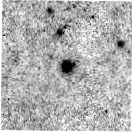
\includegraphics[width=0.3\textwidth]{ASASSN-14li_host_red}
  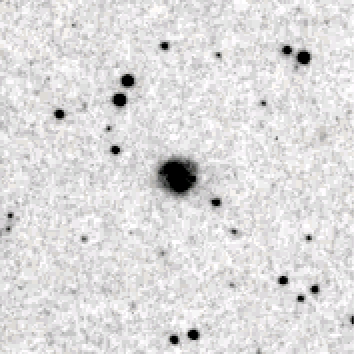
\includegraphics[width=0.3\textwidth]{AT2019qiz_host_red}
  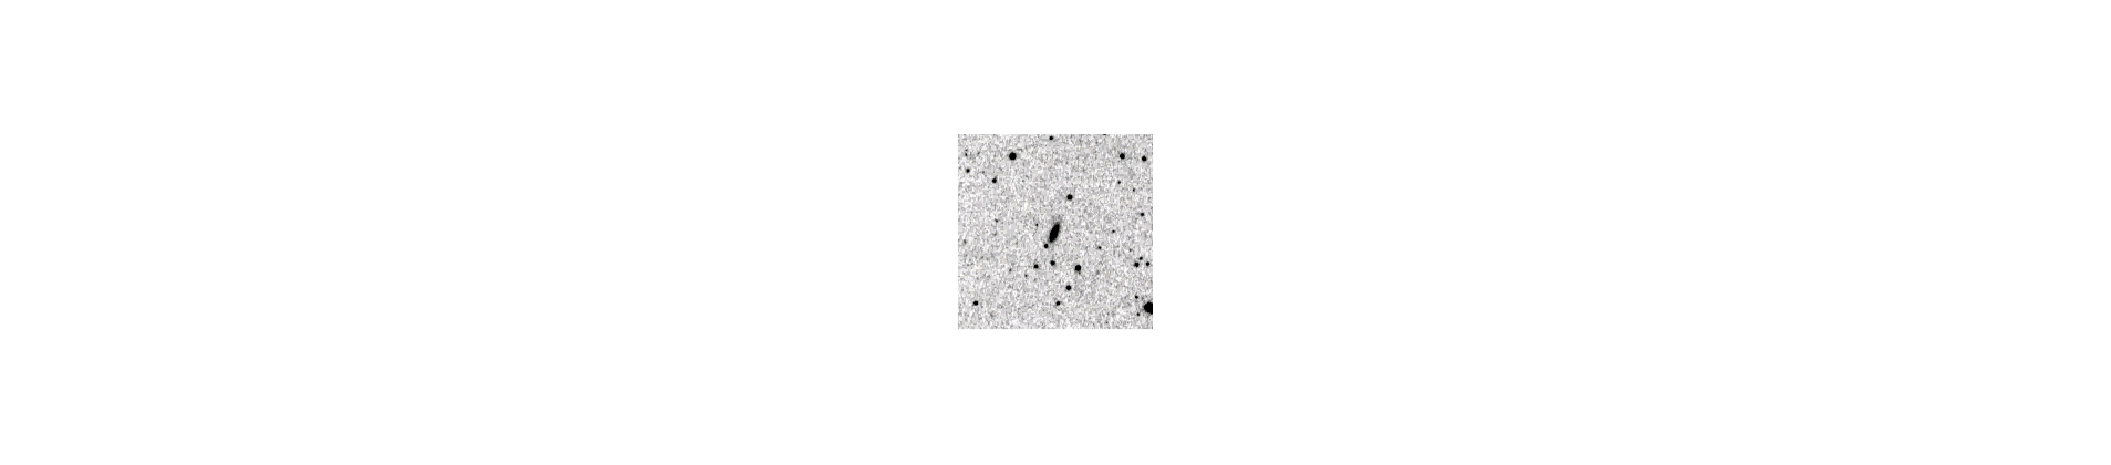
\includegraphics[width=0.3\textwidth]{iPTF16fnl_host_red}
  \caption{ASASSN-14li, AT2019qiz, and iPTF16fnl host galaxies.}
  \label{fig:xshooter_hosts}
\end{figure}

To do this, I utilised spectroscopic and photometric data on eight galaxies which hosted a tidal disruption event between 2014 and 2020. Table \ref{tab:xshooter_data} lists the targets, which were observed between September and December of 2020, with the XSHOOTER instrument on the Very Large Telescope (VLT). They are all of similar magnitude and moderate redshift, all  being located at $z<0.1$. At such distances, they occupy little real estate on a CCD (see Fig. \ref{fig:xshooter_hosts}), but the XSHOOTER instrument provides detailed, ground-based spectroscopy of the TDE hosts, with flux bins of width $\Delta\lambda=\SI{0.2}{\angstrom}$ below \SI{10200}{\angstrom} and $\Delta\lambda=\SI{0.6}{\angstrom}$ above \SI{10200}{\angstrom}. Some of the spectra featured strong telluric lines from the Earth's atmosphere, but the errors on these fluxes can be exaggerated to ensure \textsc{Bagpipes} does not overfit them, as described in \S \ref{sec:bagpipes_module}.

\begin{table}[H]
  \centering
  \begin{tabular}{l l c c r}
    TDE         & Host Galaxy             & $m$ & Morphology & $z$      \\
    \hline \hline
    ASASSN-14li & PGC 043234              & 15  & Compact    & 0.0206   \\
    ASASSN-15oi & 2MASX J20390918-3045201 & 16  & Unresolved & 0.0484   \\
    AT2018fyk   & LCRS B224721.6-450748   & 17  & Unresolved & 0.06     \\
    AT2019ahk   & 2MASX J07001137-6602251 & 17  & E+A        & 0.026211 \\
    AT2019azh   & KUG 0810+227            & 15  & E+A        & 0.022    \\
    AT2019dsg   & 2MASX J20570298+1412165 & 15  & Unresolved & 0.0512   \\
    AT2019qiz   & 2MASX J04463790-1013349 & 15  & Unresolved & 0.01513  \\
    iPTF16fnl   & Markarian 950           & 16  & E+A        & 0.018    \\
    \hline
  \end{tabular}
  \caption{
  XSHOOTER target TDEs, their host galaxies, magnitudes, host morphologies
  (if known), and redshifts, which were observed on the Very Large Telescope
  (VLT) between September and December 2020.\cite{Zwicky_1975, Jose_2014,
  Holoien_2016a, Arcavi_2015, Holoien_2016b, Wevers_2021, Cacella_2019,
  Holoien_2019, van_Velzen_2019, Perez_Torres_2019, Seibert_2019, Gezari_2016, Blagorodnova_2017}
  }
  \label{tab:xshooter_data}
\end{table}

\subsection{The Bagpipes Module}\label{sec:bagpipes_module}

\begin{figure}[H]
  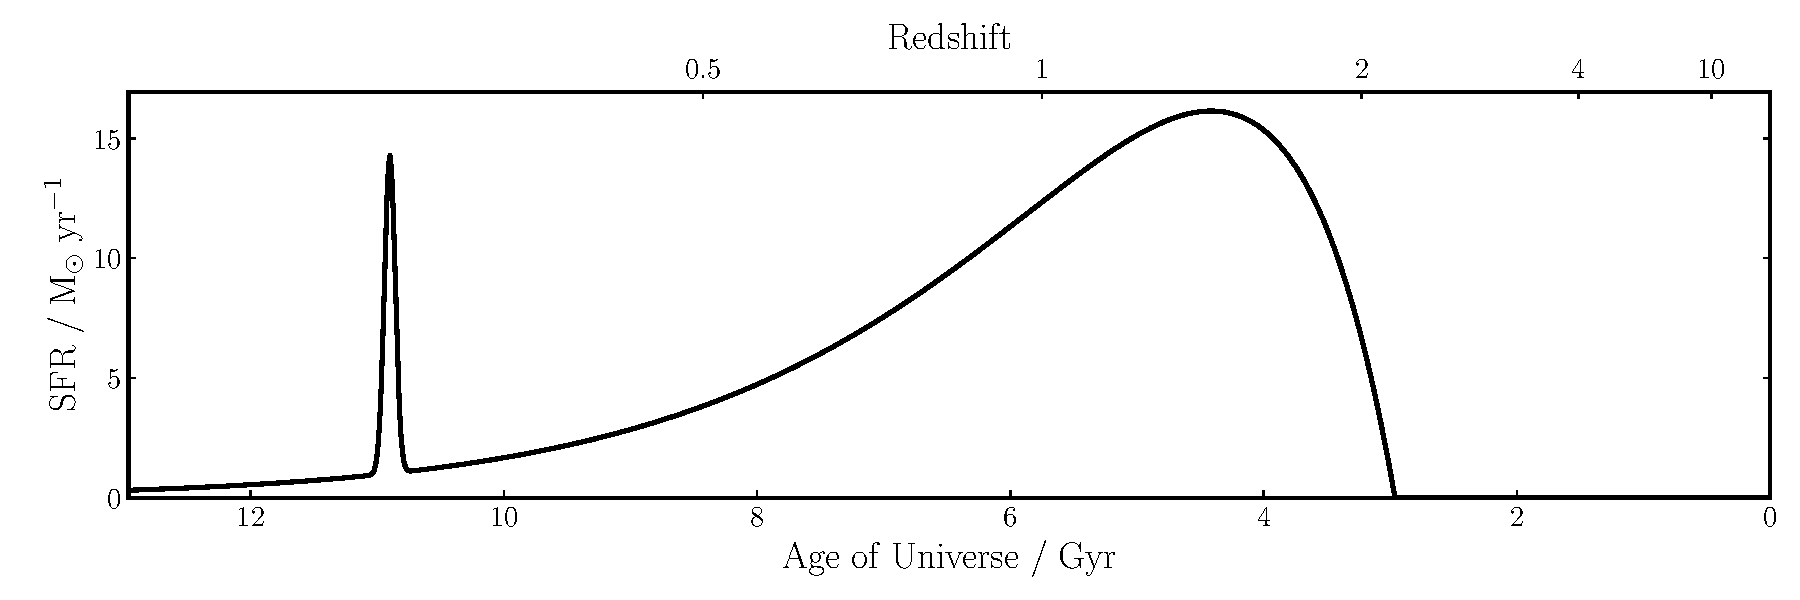
\includegraphics[width=\textwidth]{alex_model_20_sfh}
  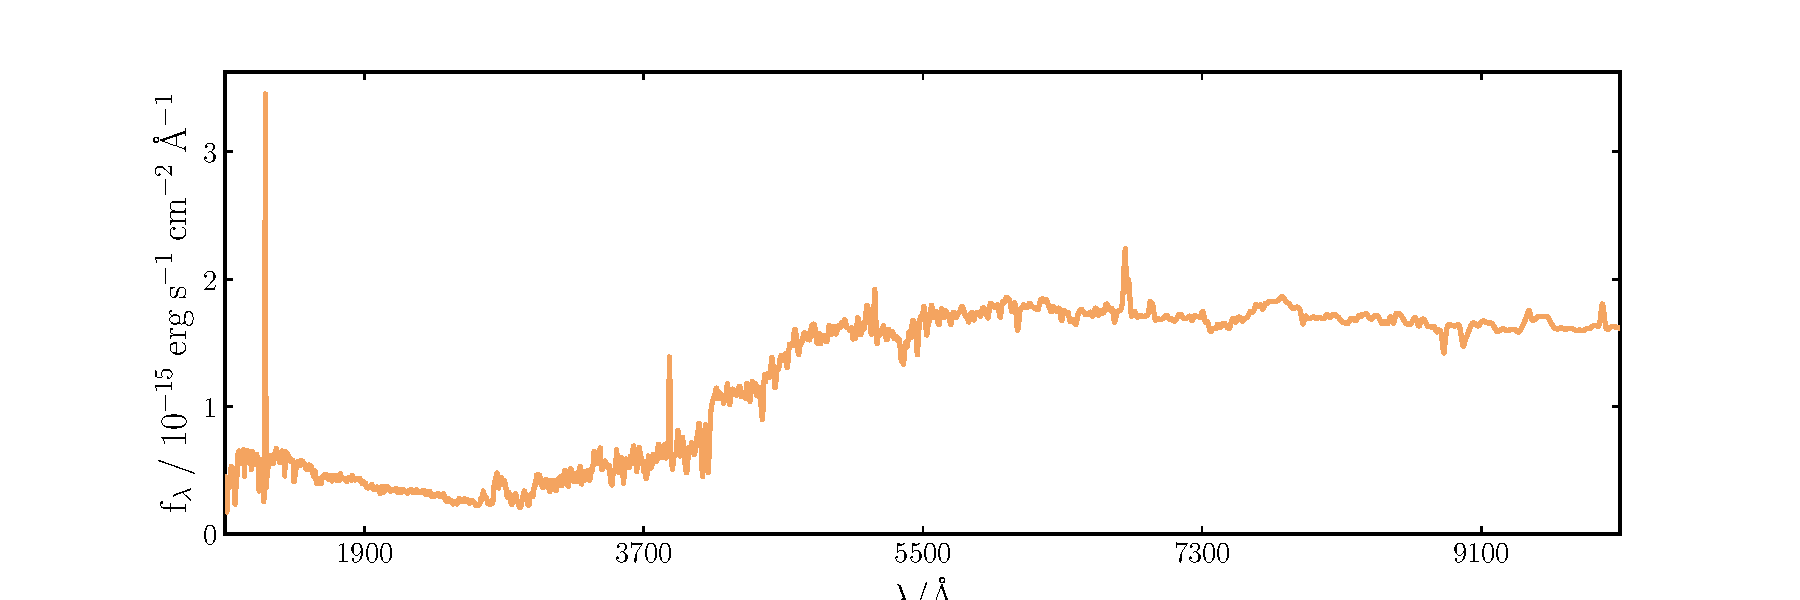
\includegraphics[width=\textwidth]{alex_model_20_spec}
  \caption{Parameterised star formation history and simulated spectrum with \textsc{Bagpipes}.}
  \label{fig:bagpipes_example_simulation}
\end{figure}

\textsc{Bagpipes} is a module for Python 3, implemented by Carnall et al. 2018. Its moniker is an acronym for Bayesian Analyses of Galaxies for Physical Inference and Parameter EStimation. \textsc{Bagpipes} constructs model galaxies from a variety of parameters, such as the form of the SFH, observed redshift, dust attenuation, and nebular emission. From this model, \textsc{Bagpipes} generates model spectral energy distributions, as they would be observed if they were real galaxies. The luminosity per unit rest-frame wavelength $L_\lambda(\lambda)$, from sum of four ``ingredients'':

\begin{itemize}
  \item The SFH, $\mathrm{SFR}(t)$, which is a linear combination of one or more of the functional forms described below.
  \item Simple stellar population models, $\mathrm{SSP}(a,\lambda,Z)$ which give the spectral energy distribution for a total stellar mass of age $a$ given by the SFH, on the basis of an initial mass function (IMF) and the metallicity of stellar population or populations.
  \item The transmission function of the ionised ISM, $T^+(a,\lambda)$ which determines how starlight is absorbed and re-emitted by hot gas regions.
  \item Finally, the transmission function of the neutral ISM, $T^0(a,\lambda)$, which determines how starlight is absorbed and remitted by cold gas and dust regions.\cite{Carnall_2018}
\end{itemize}

\noindent These are combined to give the galactic rest-frame spectrum:

\begin{equation}\label{eq:luminosity_per_rframe_wavelength}
  L_\lambda(\lambda) =
  \sum_{j=1}^{N_c} \sum_{i=1}^{N_a}
  \mathrm{SFR}_j(t_i)
  \mathrm{SSP}(a_i,\lambda,Z_j)
  T^+(a_i,\lambda)
  T^0(a_i,\lambda)
  \Delta a_i
\end{equation}

\noindent Where $i$ runs over the number of stellar age bins defined by \textsc{Bagpipes} and $j$ runs over the components of the SFH.\cite{Carnall_2018} An example spectrum from a parameterised SFH is given in Fig. \ref{fig:bagpipes_example_simulation}. The parameterised SFH, is a linear combination of one or more of the following functional forms. An exponentially decaying burst with form:

\begin{equation}\label{eq:tau_model}
  \mathrm{SFR}(t) \propto
  \begin{cases}
    \exp\left({-\frac{t-T_0}{\tau}}\right) & t > T_0, \\
    0 & t < T_0
  \end{cases}
\end{equation}

\noindent A delayed exponentially decaying component:

\begin{equation}\label{eq:delayed_model}
  \mathrm{SFR}(t) \propto
  \begin{cases}
    (t-T_0)\exp\left({-\frac{t-T_0}{\tau}}\right) & t > T_0, \\
    0 & t < T_0
  \end{cases}
\end{equation}

\noindent A lognormal form:

\begin{equation}\label{eq:lognormal_model}
  \mathrm{SFR}(t) \propto
  \frac{1}{t\sqrt{2\pi\tau^2}}
  \exp\left({-\frac{\left(\ln{t-t_0}\right)^2}{2\tau^2}}\right)
\end{equation}

\noindent Defined by Gladders et al. 2013, where $t$ is the elapsed time since the big bang, $t_0$ is the logarithmic decay time, and $\tau$ sets rise and decay timescale.\cite{Gladders_2013} \textsc{Bagpipes}, however, parameterises this as $t_{max}$, the time since the big bang at the peak rate of star formation and $2\sigma$, the full width at half maximum (FWHM) of the star formation rate.\cite{Carnall_2019b} Finally, \textsc{Bagpipes} allows a more versatile double power law parameterisation:

\begin{equation}\label{eq:dblplaw_model}
  \mathrm{SFR}(t)\propto
  \left[
  \left(\frac{t}{\tau}\right)^{\alpha} +
  \left(\frac{t}{\tau}\right)^{-\beta}
  \right]
  ^{-1}
\end{equation}

\noindent Which usefully decouples the rising $\alpha$ and falling $\beta$ slopes of the star formation, at the expense of an additional parameter in a fit which is already of high dimensionality and of increased computational resources.\cite{Carnall_2018} Each of the above parameterisations include a parameter each for the total stellar mass $M_\star$ formed by the component and the metallicity $Z$ of the stars formed. It is possible to include ``bursts'' of fixed mass such that:

\begin{equation}
  \mathrm{SFR}(t)\propto
  M_\star \delta(t-T_0)
\end{equation}

\noindent As a matter of semantics, such ``bursts'' are not necessarily synonymous with the type of ``starburst'' activity for which we are searching. The starburst component may take one of any of these forms.

Global parameters for the entire model galaxy include the observed redshift $z_obs$, the velocity dispersion $\sigma_v$ of the stellar population,the logarithm of the nebular ionisation rate $\log{U}$, and the extinction $A_V$ in magnitudes due to dust in the galaxy, which contribute to the summation in Eq. \ref{eq:luminosity_per_rframe_wavelength}.

\textbf{Mention dust extinction curve (type) here!}

\begin{figure}
  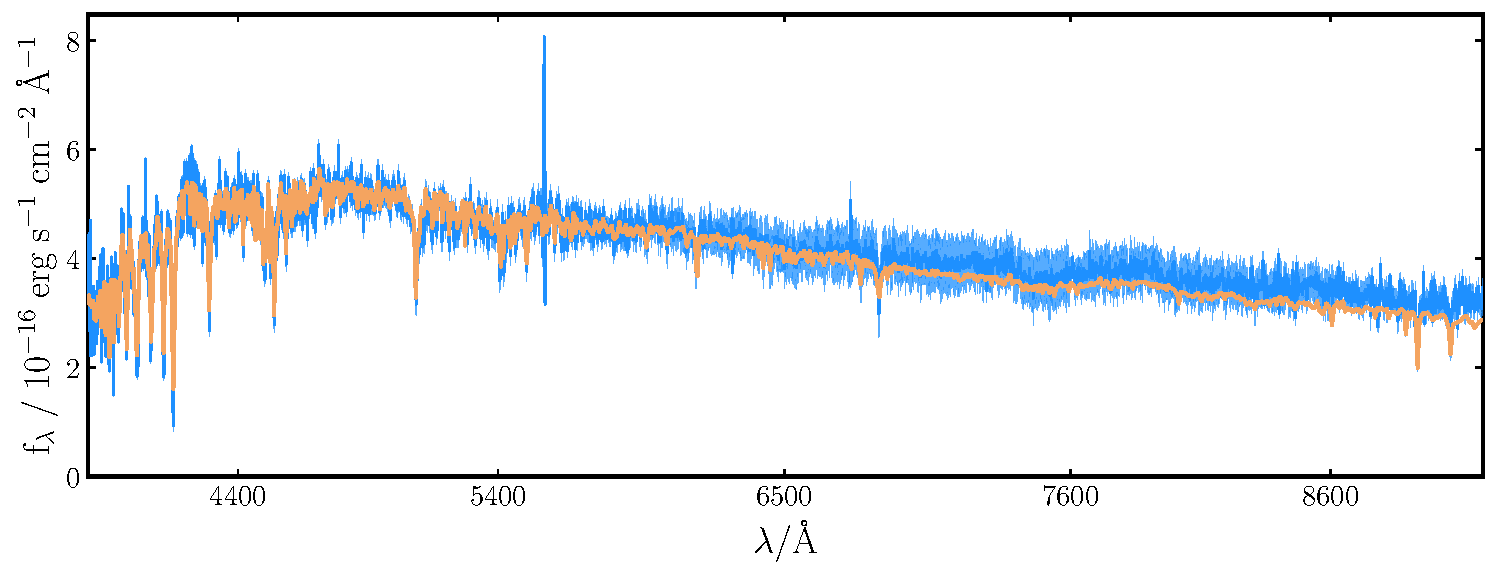
\includegraphics[width=\textwidth]{host_hyz_specwerr_fit}
  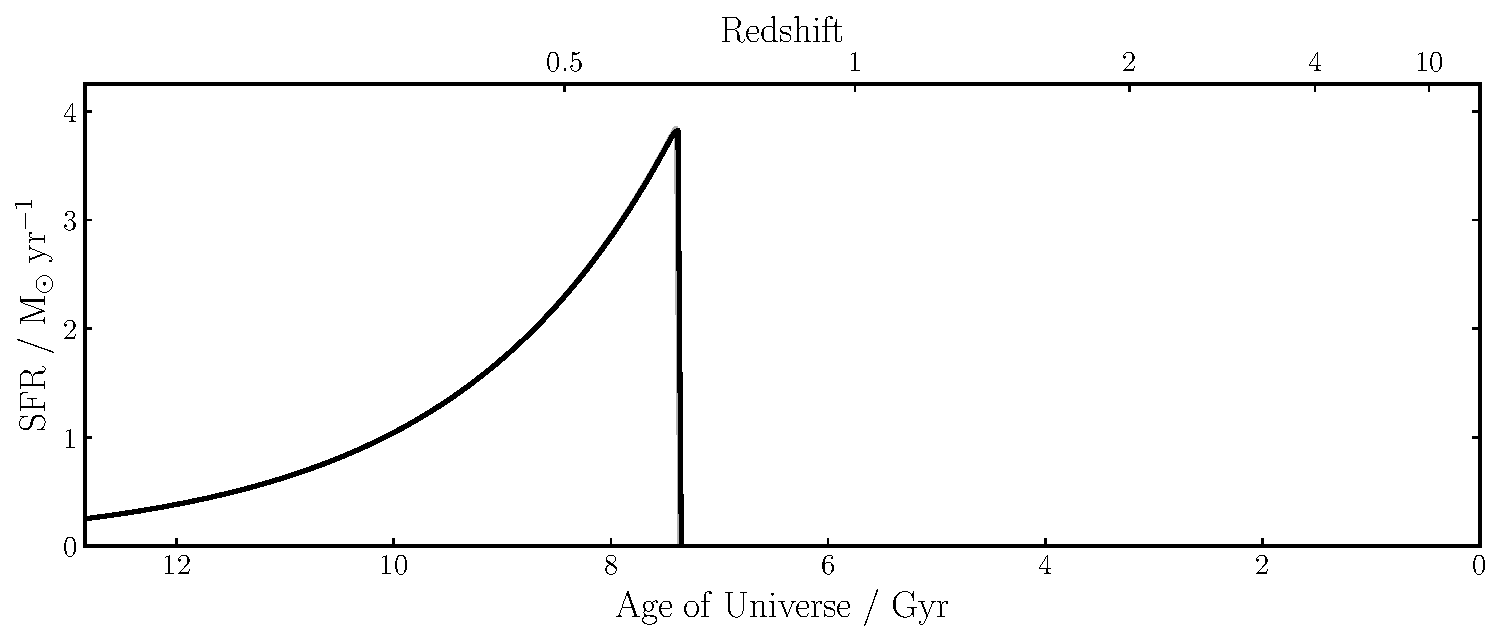
\includegraphics[width=\textwidth]{host_hyz_specwerr_sfh}
  \caption{Observed (blue) spectrum, fitted (orange) spectrum, and inferred star formation history with \textsc{Bagpipes}.}
  \label{fig:bagpipes_example_fit}
\end{figure}

The real power of \textsc{Bagpipes}, however, is that it can also do the inverse: take in an observed spectrum and infer the most likely star formation history for that galaxy. By utilising Bayes' Theorem for some new data $\mathcal{D}$, a hypothesis $\mathcal{H}$ with parameter vector:

\begin{equation}\label{eq:bayes_theorem}
  P(\Theta|\mathcal{D},\mathcal{H}) =
  \frac
  {P(\mathcal{D}|\Theta,\mathcal{H})P(\Theta|\mathcal{H})}
  {P(\mathcal{D}|\mathcal{H})}
\end{equation}

And the \textsc{LINEST} linear algebra sampling method to determine the probability that a model galaxy spectrum described by Eq. \ref{eq:luminosity_per_rframe_wavelength} is a fit for the observed spectrum, \textsc{Bagpipes} produces a posterior distribution of SFHs and their associated parameters.

\subsection{Stellar Population Fitting}\label{sec:stellar_population_fitting}

\begin{table}
  \centering
  \begin{tabular}{c c r r r}
    Spectral Type & $M/M_\odot$ & $\lambda_{peak}$     & MS Lifetime   & No. Density \\
    \hline \hline
    O5            &	40          & \SI{725}{\angstrom}  & \SI{1}{Myr}   & 1           \\
    B0            &	15          & \SI{1035}{\angstrom} & \SI{11}{Myr}  & 5           \\
    A0            &	3.5         & \SI{2898}{\angstrom} & \SI{440}{Myr} & 25          \\
    F0            &	1.7         & \SI{3864}{\angstrom} & \SI{2.7}{Gyr} & 63          \\
    G0            &	1.1         & \SI{4830}{\angstrom} & \SI{8}{Gyr}   & 100         \\
    K0            &	0.8         & \SI{5796}{\angstrom} & \SI{17}{Gyr}  & 630         \\
    M0            &	0.5         & \SI{8280}{\angstrom} & \SI{56}{Gyr}  & 800         \\
    \hline
  \end{tabular}
  \caption{Typical masses, temperatures, and main-sequence lifetimes for seven Harvard spectral subtypes. Number densities per \SI{10000}{\cubic\parsec} for each subtype's respective super-type are adapted from Glenn et al. 2001.\cite{Glenn_2001}}
  \label{tab:star_lifetimes_densities}
\end{table}

Many of the challenges in fitting spectra to SFHs are due to the limitations of stellar population fitting, whereby the total luminosity and the ratio of blue to red stars constituent in a host galaxy is used to infer the age of stellar formation components. The main sequence lifetime of a star is given by\cite{Prialnik_2010}:

\begin{equation}
  T_{MS} \propto \left(\frac{M}{M_\odot}\right)^{-2}
\end{equation}

\noindent From this we obtain the typical main-sequence lifetimes for stars of different Harvard spectral classifications, given in Table \ref{tab:star_lifetimes_densities}. From this data, the limitations of stellar population fitting are immediately apparent. Due to the inverse power law relationship between mass and main-sequence lifetime, small reductions in the initial mass (and therefore, main-sequence temperature) of stars result in dramatic increases in main-sequence lifetime. While on the main-sequence, the luminosity and colour of these long-lived stars varies little.\cite{Prialnik_2010} If, for example, the hottest stars in a stellar population are G-type stars, then stellar population fitting may reasonably find that population to be anywhere between \SI{3}{Gyr} and \SI{11}{Gyr} old. This kind of temporal resolution is comparable to the age of the universe, but star formation rates are believed to vary on much smaller timescales.\cite{Kauffmann_2003c} If star forming processes create new stars with initial masses according to some initial mass function (IMF), then star formation of sufficient total mass formed will always create some stars of each spectral type. But once the population of A-type stars, with lifetimes on the order of \SI{100}{Myr}, die out completely, it becomes increasingly difficult to pinpoint the precise age of that formation.

Indeed, observations by Glenn et al. 2001 reproduced in Table \ref{tab:star_lifetimes_densities} show that our own Milky Way, despite being a relatively young, blue galaxy, is nevertheless mostly populated by cool red dwarves, whose lifetimes are many times that of the current age of the universe.

\section{Metal and Nebular Emission Lines}

Astrophysics of gaseous nebulae

\section{Blind Fitting with \textsc{Bagpipes}}\label{sec:blind_fitting}
Emphasize importance of computational speed. Necessity of Chi-squared selection
\subsection{R1: Wide Parameter Space with Two Components}\label{sec:r1}
For my first fitting run, I tried to first establish the functional form of the
old, bulk star formation, and then determine whether or not a more recent burst
improved the fit. I first fit each of the following functions:

\begin{tabular}{| c | c |}
  \hline
  \multicolumn{2}{| c |}{$SFR=e^{t/\tau}$} \\
  \hline
  $t$ & (3.5, 10.0) \\
  $\tau$ & (0.1, 2.0) \\
  $\log_{10}(\sfrac{M}{M_\odot})$ & (0.0, 15.0) \\
  $\sfrac{Z}{Z_\odot}$ & (0.0, 2.5) \\
  \hline
\end{tabular}

\begin{tabular}{| c | c |}
  \hline
  \multicolumn{2}{| c |}{$SFR=te^{\sfrac{-t}{\tau}}$} \\
  \hline
  $t$ & (3.5, 10.0) \\
  $\tau$ & (0.1, 2.0) \\
  $\log_{10}(\sfrac{M}{M_\odot})$ & (0.0, 15.0) \\
  $\sfrac{Z}{Z_\odot}$ & (0.0, 2.5) \\
  \hline
\end{tabular}

\begin{tabular}{| c | c |}
  \hline
  \multicolumn{2}{| c |}{$SFR=lognormal$} \\
  \hline
  $t_{max}$ & (3.5, 10.5) \\
  $2\sigma$ & (0.1, 5.0) \\
  $\log_{10}(\sfrac{M}{M_\odot})$ & (0.0, 15.0) \\
  $\sfrac{Z}{Z_\odot}$ & (0.0, 2.5) \\
  \hline
\end{tabular}

\begin{tabular}{| c | c |}
  \hline
  \multicolumn{2}{| c |}{Global Priors} \\
  \hline
  Dust Type & Calzetti \\
  $A_V$ & (0.0, 1.0) \\
  $z$ & (0.0, 0.1) \\
  $T_{bc}$ & (0.005, 0.015) \\
  $\sigma_{v}$ & (150.0, 200.0) \\
  \hline
\end{tabular}

Once the best-fit functional form of the old, bulk star formation is determined, a new fit is run with that form in linear combination with a delta function, with priors:

\begin{tabular}{| c | c |}
  \hline
  \multicolumn{2}{| c |}{$SFR=\delta_a(t)$} \\
  \hline
  $a$ & (0.1, $a_{low}$) \\
  $\log_{10}(\sfrac{M}{M_\odot})$ & (0.0, 15.0) \\
  $\sfrac{Z}{Z_\odot}$ & (0.0, 2.5) \\
  \hline
\end{tabular}
\subsection{R2 \& R3: Iterative Fitting}\label{sec:r2_and_r3}
One of the three functional forms above \textit{or} the more versatile double power law function:

\begin{equation}
  \mathrm{SFR}(t) \propto \left[ \left(\frac{t}{\tau}\right)^{\alpha} + \left(\frac{t}{\tau}\right)^{-\beta} \right]^{-1}
\end{equation}

With priors:

\begin{tabular}{| c | c |}
  \hline
  \multicolumn{2}{| c |}{$\mathrm{SFR}(t)\propto\left[\left(\sfrac{t}{\tau}\right)^{\alpha}+\left(\sfrac{t}{\tau}\right)^{-\beta} \right]^{-1}$} \\
  \hline
  $\tau$ & (0.0, 15.0) \\
  $\alpha$ & (0.0, 10.0) \\
  $\beta$ & (0.0, 10.0) \\
  $\log_{10}(\sfrac{M}{M_\odot})$ & (0.0, 15.0) \\
  $\sfrac{Z}{Z_\odot}$ & (0.0, 2.5) \\
  \hline
\end{tabular}

And with an exponentially decaying burst, the age of which is allowed to vary over a much larger parameter space:

\begin{tabular}{| c | c |}
  \hline
  \multicolumn{2}{| c |}{$SFR=e^{t/\tau}$} \\
  \hline
  $t$ & (0.0, 10.0) \\
  $\tau$ & (0.1, 2.0) \\
  $\log_{10}(\sfrac{M}{M_\odot})$ & (0.0, 15.0) \\
  $\sfrac{Z}{Z_\odot}$ & (0.0, 2.5) \\
  \hline
\end{tabular}
\subsection{Selecting Physically Reasonable Priors}\label{sec:prior_selection}

Velocity dispersion of constituent stars is allowed to vary between

The ionization parameter for nebular emission is allowed to vary between logU=-4 and logU=-2, a very low and very high rate of (molecular?) ionization.

The lifetime of the stellar birth clouds was chosen to be a normal distribution about ${t_{BC}=17Myr}$ with ${\sigma=4Myr}$, consistent with typical cloud lifetimes in the Milky Way, as determined by Murray 2011\cite{Murray_2011}.
\subsection{R4: Fixed Old Component, Free Burst Component}\label{sec:r4}
Quenching at Cosmic Noon
\begin{tabular}{| c | c |}
  \hline
  \multicolumn{2}{| c |}{$SFR=e^{t/\tau}$} \\
  \hline
  $t$ & (7.5, 12.5) \\
  $\tau$ & (0.5, 2.0) \\
  $\log_{10}(\sfrac{M}{M_\odot})$ & (5.0, 12.5) \\
  $\sfrac{Z}{Z_\odot}$ & (0.0, 2.5) \\
  \hline
\end{tabular}

\begin{tabular}{| c | c |}
  \hline
  \multicolumn{2}{| c |}{$SFR=te^{\sfrac{-t}{\tau}}$} \\
  \hline
  $t$ & (7.5, 12.5) \\
  $\tau$ & (0.1, 2.0) \\
  $\log_{10}(\sfrac{M}{M_\odot})$ & (5.0, 12.5) \\
  $\sfrac{Z}{Z_\odot}$ & (0.0, 2.5) \\
  \hline
\end{tabular}

\begin{tabular}{| c | c |}
  \hline
  \multicolumn{2}{| c |}{$SFR=lognormal$} \\
  \hline
  $t_{max}$ & (1.0, 6.0) \\
  $2\sigma$ & (0.1, 3.0) \\
  $\log_{10}(\sfrac{M}{M_\odot})$ & (5.0, 12.5) \\
  $\sfrac{Z}{Z_\odot}$ & (0.0, 2.5) \\
  \hline
\end{tabular}

\begin{tabular}{| c | c |}
  \hline
  \multicolumn{2}{| c |}{$\mathrm{SFR}(t)\propto\left[\left(\sfrac{t}{\tau}\right)^{\alpha}+\left(\sfrac{t}{\tau}\right)^{-\beta} \right]^{-1}$} \\
  \hline
  $\tau$ & (0.0, 4.5) \\
  $\alpha$ & (5.0, 10.0) \\
  $\beta$ & (5.0, 10.0) \\
  $\log_{10}(\sfrac{M}{M_\odot})$ & (5.0, 12.5) \\
  $\sfrac{Z}{Z_\odot}$ & (0.0, 2.5) \\
  \hline
\end{tabular}

And an exponentially declining burst with priors:

\begin{tabular}{| c | c |}
  \hline
  \multicolumn{2}{| c |}{$SFR=e^{t/\tau}$} \\
  \hline
  $t$ & (0.0, 3.5) \\ %Gyr, lifetime of F type stars
  $\tau$ & (0.1, 2.0) \\
  $\log_{10}(\sfrac{M}{M_\odot})$ & (0.0, 12.5) \\
  $\sfrac{Z}{Z_\odot}$ & (0.0, 2.5) \\
  \hline
\end{tabular}

\begin{tabular}{| c | c |}
  \hline
  \multicolumn{2}{| c |}{Global Priors} \\
  \hline
  Dust Type & Calzetti \\
  $z$ & ($z_{obs}-0.001$, $z_{obs}+0.001$) \\ % z varies tight_layout around z_obs.
  $\sigma_{v}$ & (50.0, 450.0) \\ % Constrained by Faber-Jackson. TODO: Lookup Minkowski 1962!
  $T_{bc}$ & (0.013, 0.021) \\  % Constraints from Murray 2011.
  $A_V$ & (0.0, 2.0) \\
  $\log{U}$ & (-4.0, -2.0) \\
  \hline
\end{tabular}
\section{Application to XSHOOTER Data}\label{sec:tde_fitting}
\section{Results \& Discussion}\label{sec:results_and_discussion}

Here follows a discussion of the R4 priors applied to the eight XSHOOTER targets, their inferred star formation histories for the $\mathrm{reduced-}\chi^2$ best fit spectra, and the posterior distributions of their parameters, with comparison to established literature on the targets.

\subsection{ASASSN-14li, $z=0.0206$}\label{sec:ASASSN-14li}
\begin{figure}[h!]
\centering
  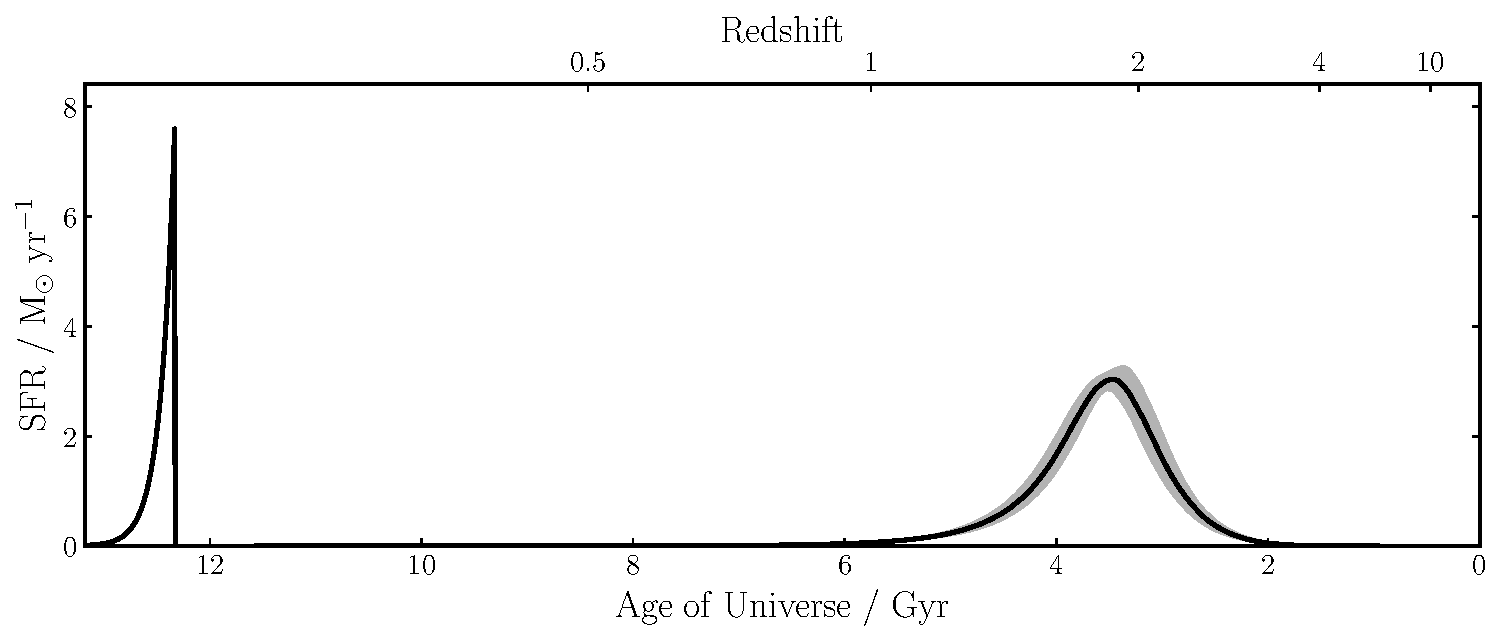
\includegraphics[width=0.9\textwidth]{../pipes/plots/r4_dblplaw_burst/ASASSN14li_sfh.pdf}
  \caption{Observed and fitted spectrum for the host of ASASSN-14li, and posterior SFH.}
  \label{}
\end{figure}

A very important discovery was made with ASASSN-14li.Initially identified in the optical, this is one of the few TDEs toshow evidence of both thermal and non-thermal components.ASASSN-14li was discovered by the All-Sky AutomatedSurvey for Supernovae(ASAS-SN; Shappee et al.2014)on2014 November 22 at the center of the nearby(z=0.0206,D=90.3 Mpc)post-starburst galaxy PGC 043234(Holoien et al.2016). PGC 043234 appears to be the remnant of a recentmerger that likely hosted a low-luminosity Type II AGN priorto the TDE(Prieto et al.2016). Holoien et al.(2016)present theoptical, UV, and X-ray properties of the event, followed byadditional X-ray(Miller et al.2015; Brown et al.2016),UV(Cenko et al.2016), radio(Alexander et al.2016; van Velzenet al.2016, and this work), and mid-IR(Jiang et al.2016)studies.\cite{Romero_Canizales_2016}


\newpage
\subsection{ASASSN-15oi, $z=0.0484$}\label{sec:ASASSN-15oi}
\begin{figure}[h!]
\centering
  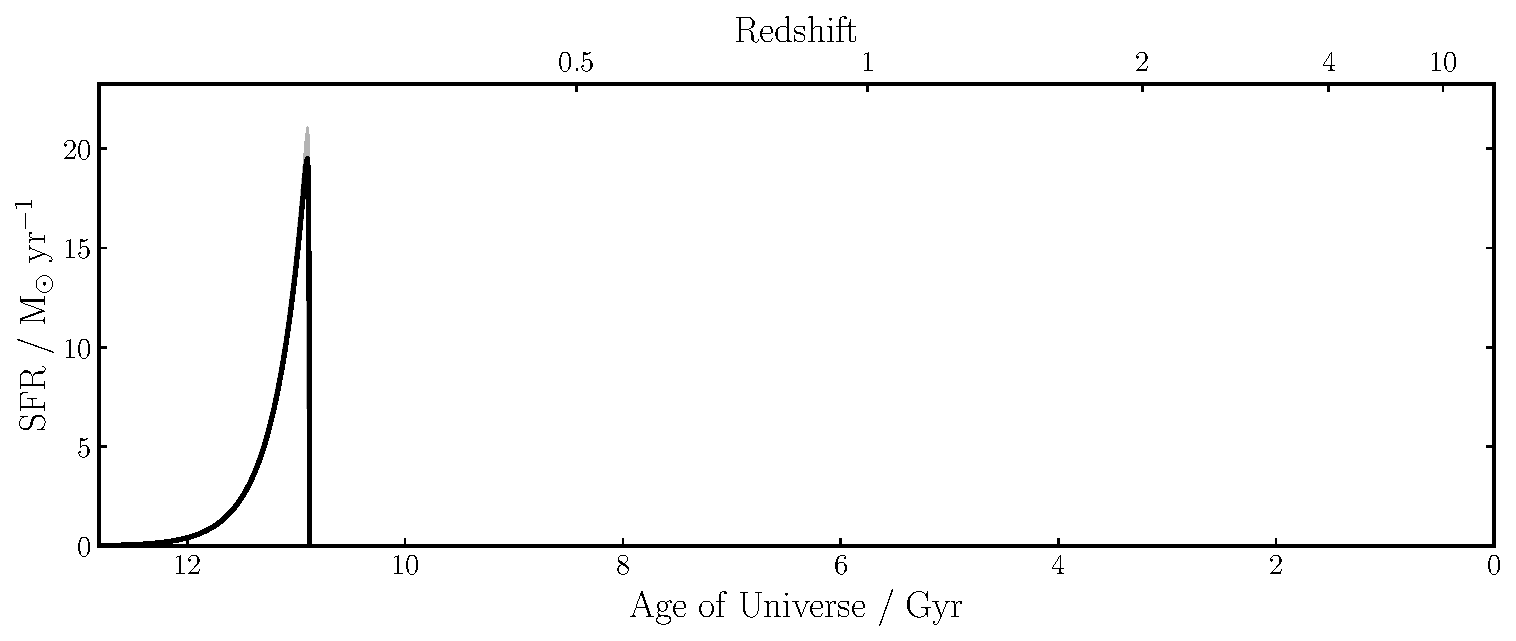
\includegraphics[width=0.9\textwidth]{../pipes/plots/r4_dblplaw_burst/ASASSN15oi_sfh.pdf}
  \caption{Observed and fitted spectrum for the host of ASASSN-15oi, and posterior SFH.}
  \label{}
\end{figure}

Although the redshift was originally reported as $z=0.02$, later spectra showed that the redshift of the host galaxy is $z=0.0484$, which was used in this fit.\cite{Arcavi_2015, Holoien_2016b}

\newpage
\subsection{AT2018fyk, $z=0.06$}\label{sec:AT2018fyk}
\begin{figure}[h!]
\centering
  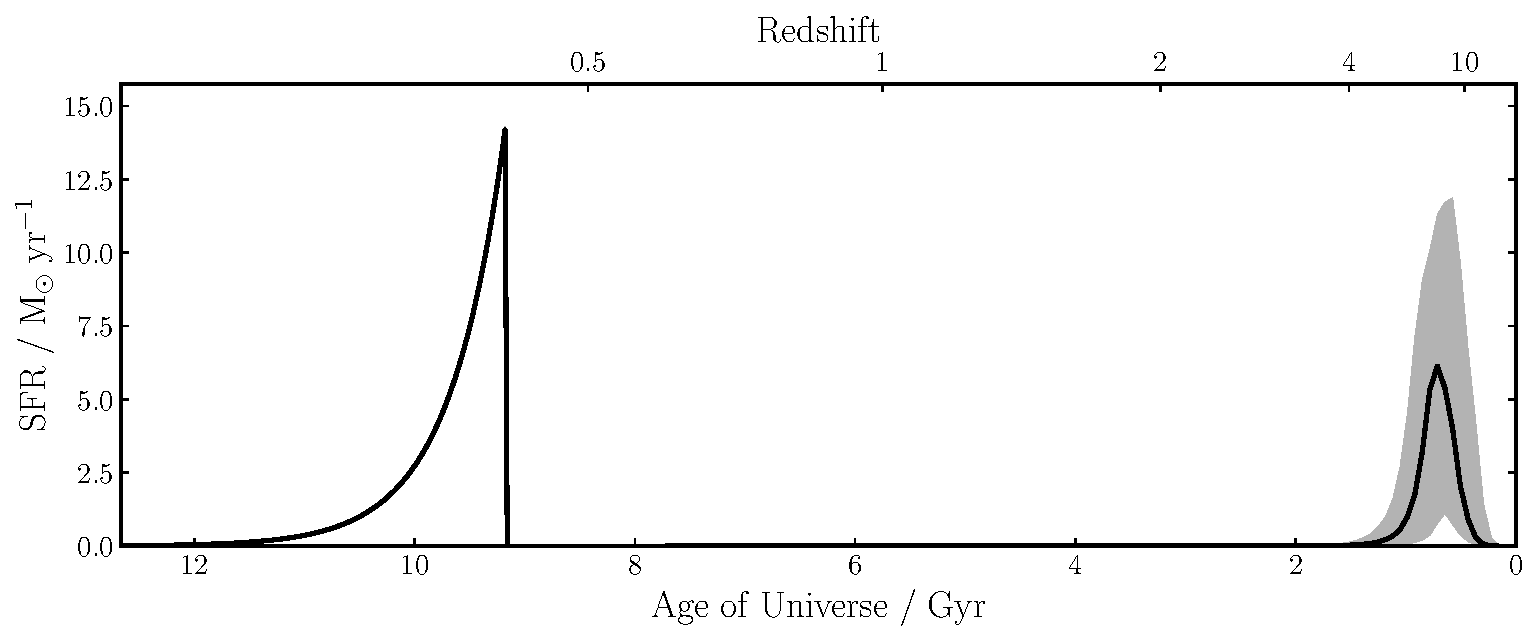
\includegraphics[width=0.9\textwidth]{../pipes/plots/r4_dblplaw_burst/AT2018fyk_sfh.pdf}
  \caption{Observed and fitted spectrum for the host of ASASSN-15oi, and posterior SFH.}
  \label{}
\end{figure}


Note that Wevers et al. 2021 gives this redshift as 0.059

\newpage
\subsection{AT2019ahk, $z=0.026211$}\label{sec:AT2019ahk}
\begin{figure}[h!]
\centering
  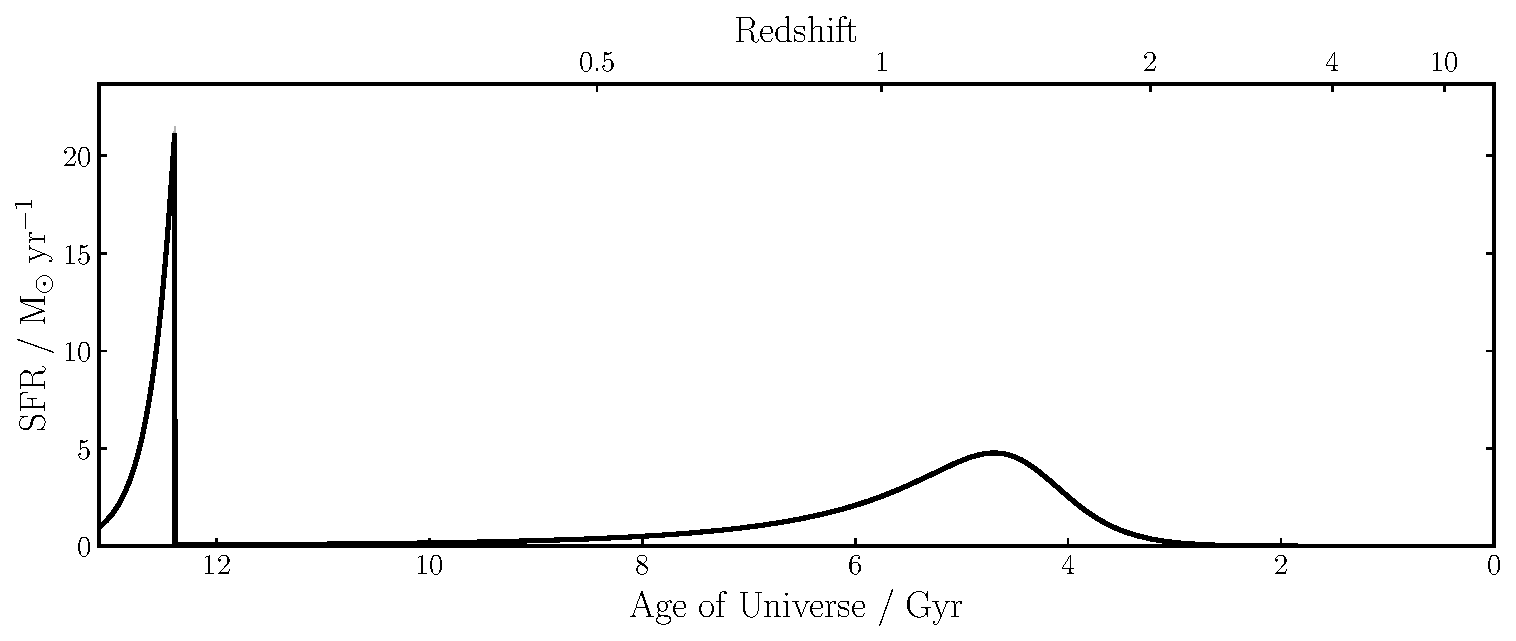
\includegraphics[width=0.9\textwidth]{../pipes/plots/r4_dblplaw_burst/AT2019ahk_sfh.pdf}
  \caption{Observed and fitted spectrum for the host of ASASSN-15oi, and posterior SFH.}
  \label{}
\end{figure}


\newpage
\subsection{AT2019azh, $z=0.022$}\label{sec:AT2019azh}
\begin{figure}[h!]
\centering
  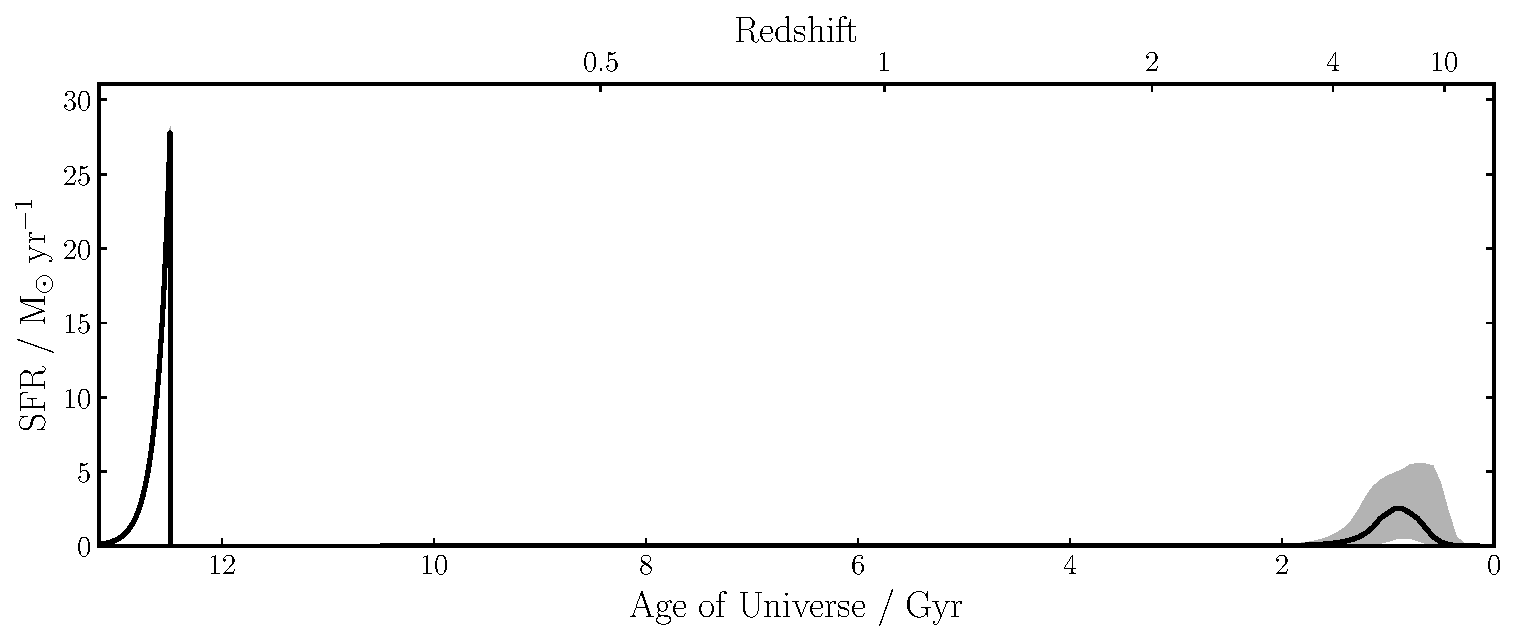
\includegraphics[width=0.9\textwidth]{../pipes/plots/r4_dblplaw_burst/AT2019azh_sfh.pdf}
  \caption{Observed and fitted spectrum for the host of ASASSN-15oi, and posterior SFH.}
  \label{}
\end{figure}


\newpage
\subsection{AT2019dsg, $z=0.0512$}\label{sec:AT2019dsg}
\begin{figure}[h!]
\centering
  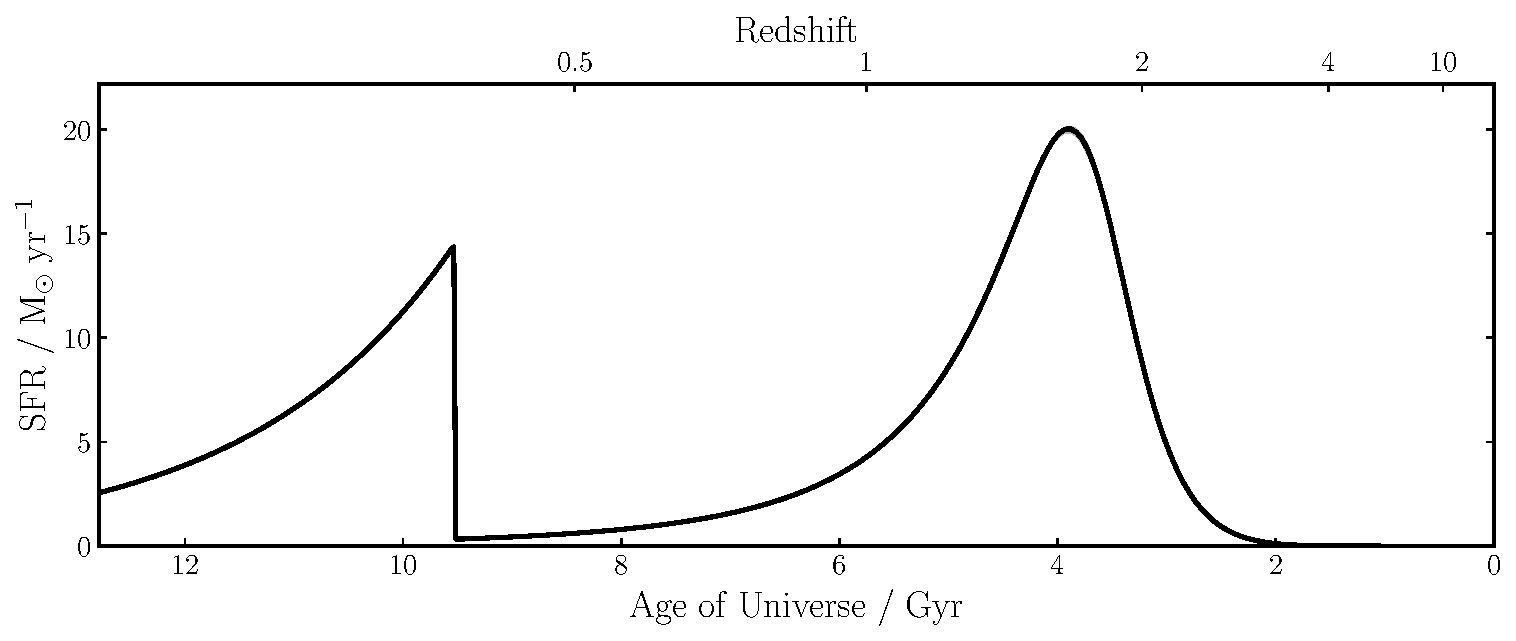
\includegraphics[width=0.9\textwidth]{../pipes/plots/r4_dblplaw_burst/AT2019dsg_sfh.pdf}
  \caption{Observed and fitted spectrum for the host of ASASSN-15oi, and posterior SFH.}
  \label{}
\end{figure}


\newpage
\subsection{AT2019qiz, $z=0.01513$}\label{sec:AT2019qiz}
\begin{figure}[h!]
\centering
  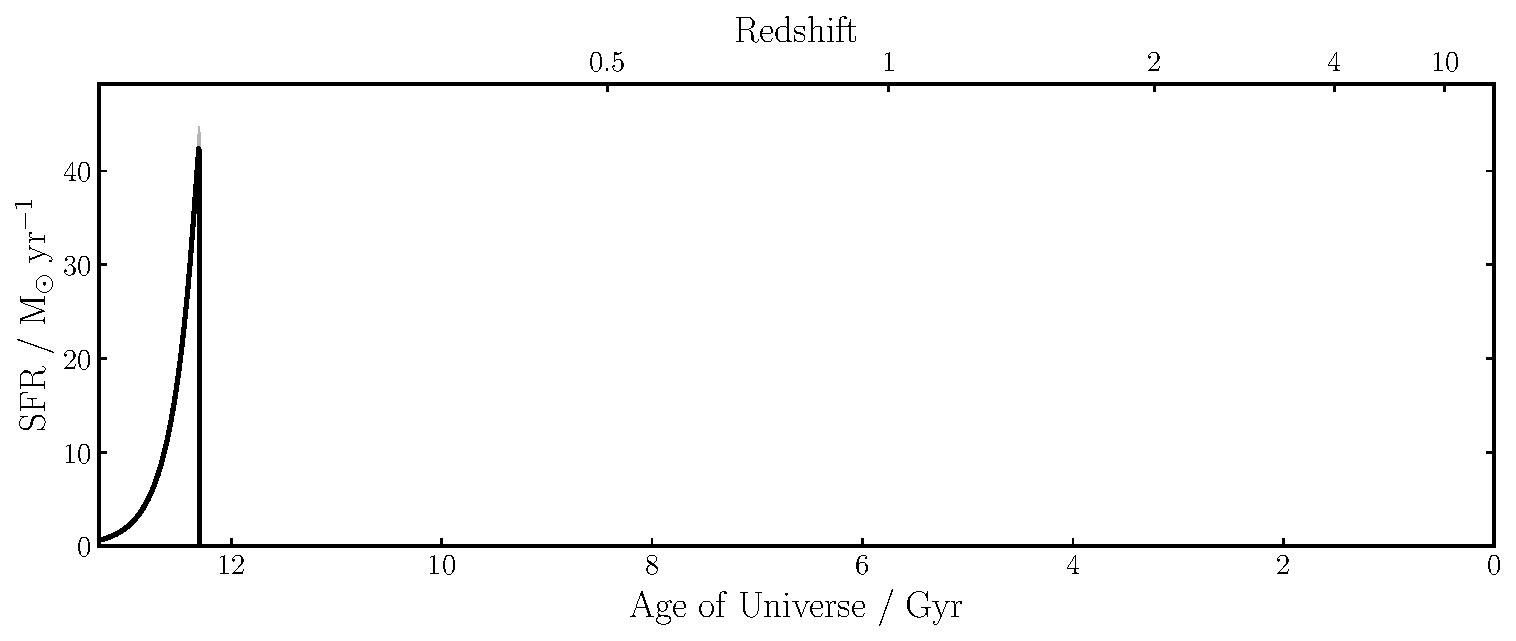
\includegraphics[width=0.9\textwidth]{../pipes/plots/r4_dblplaw_burst/AT2019qiz_sfh.pdf}
  \caption{Observed and fitted spectrum for the host of ASASSN-15oi, and posterior SFH.}
  \label{}
\end{figure}


\newpage
\subsection{iPTF16fnl, $z=0.018$}\label{sec:iPTF16fnl}
\begin{figure}[h!]
\centering
  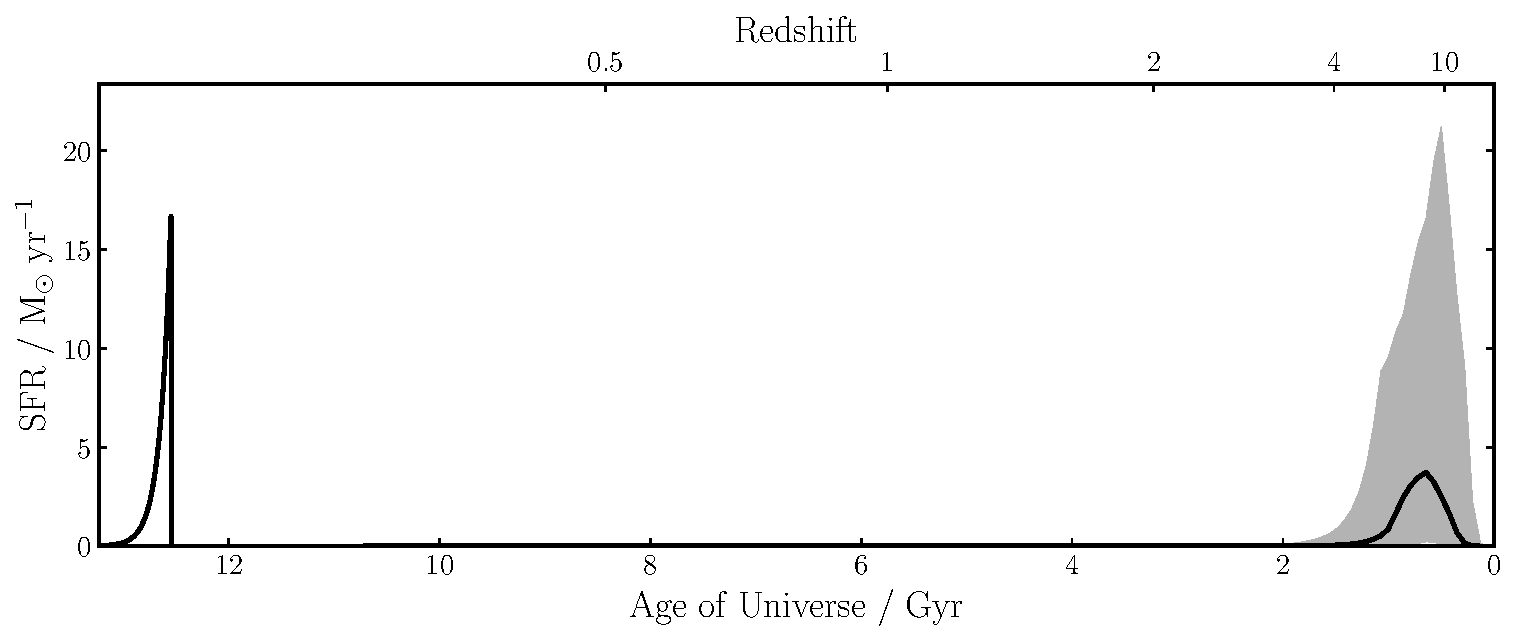
\includegraphics[width=0.9\textwidth]{../pipes/plots/r4_dblplaw_burst/iPTF16fnl_sfh.pdf}
  \caption{Observed and fitted spectrum for the host of ASASSN-15oi, and posterior SFH.}
  \label{}
\end{figure}

Important to note that Blagorodnova et al. 2017 estimates this redshift to be $z=0.016328$, although this fit was run with $z=0.018$.\cite{Blagorodnova_2017}

\section{Conclusion}\label{sec:conclusion}
\begin{itemize}
  \item Summary
  \item Future Applications
\end{itemize}
\section{Acknowledgements}\label{sec:acknowledgements}

Special thanks to Andy Lawrence, professor at the Royal Observatory Edinburgh, for his support and advice throughout this project. Thanks also to Philip Short, a PhD candidate at the University of Edinburgh, for his preparation of the XSHOOTER data and for participating in my blind fitting trials. Thanks to Patrick Smith, for endowing me with a love of empiricism in my formative school years. And finally, thanks to my father, who even before I could stand, took me for walks under the stars.

\printbibliography

% \begin{figure}[h!]
% \centering
%   \includegraphics[width=0.9\textwidth]{../pipes/plots/priors/phil_model_01_sfh.pdf}
%   \includegraphics[width=0.9\textwidth]{../pipes/plots/lognormal_noburst/phil_model_01_sfh.pdf}
%   \includegraphics[width=0.9\textwidth]{../pipes/plots/wide_lognormal_burst/phil_model_01_sfh.pdf}
%   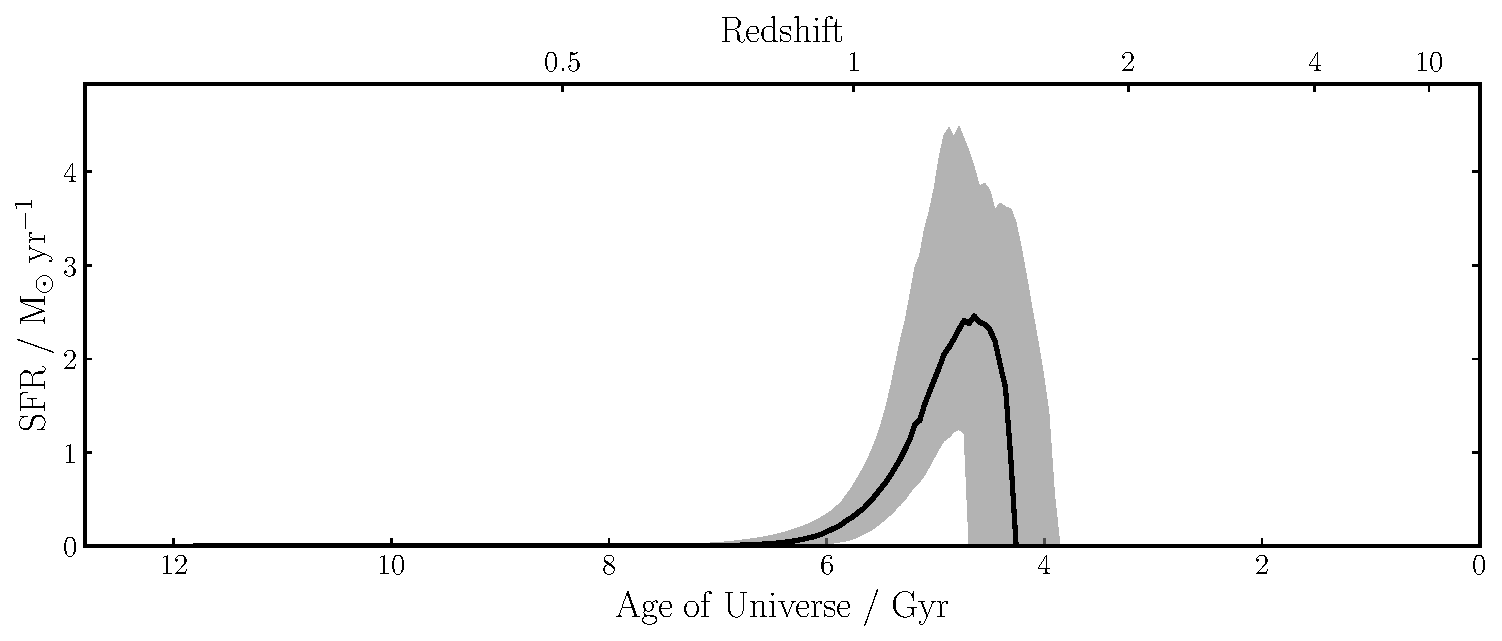
\includegraphics[width=0.9\textwidth]{../pipes/plots/lognormal_burst_final/phil_model_1_sfh.pdf}
%   \caption{A priori and posterior SFH.}
%   \label{}
% \end{figure}
%
% \newpage
% \begin{figure}[h!]
%   \centering
%   \includegraphics[width=0.9\textwidth]{../pipes/plots/priors/phil_model_02_sfh.pdf}
%   \includegraphics[width=0.9\textwidth]{../pipes/plots/exponential_burst/phil_model_02_sfh.pdf}
%   \includegraphics[width=0.9\textwidth]{../pipes/plots/wide_dblplaw_burst/phil_model_02_sfh.pdf}
%   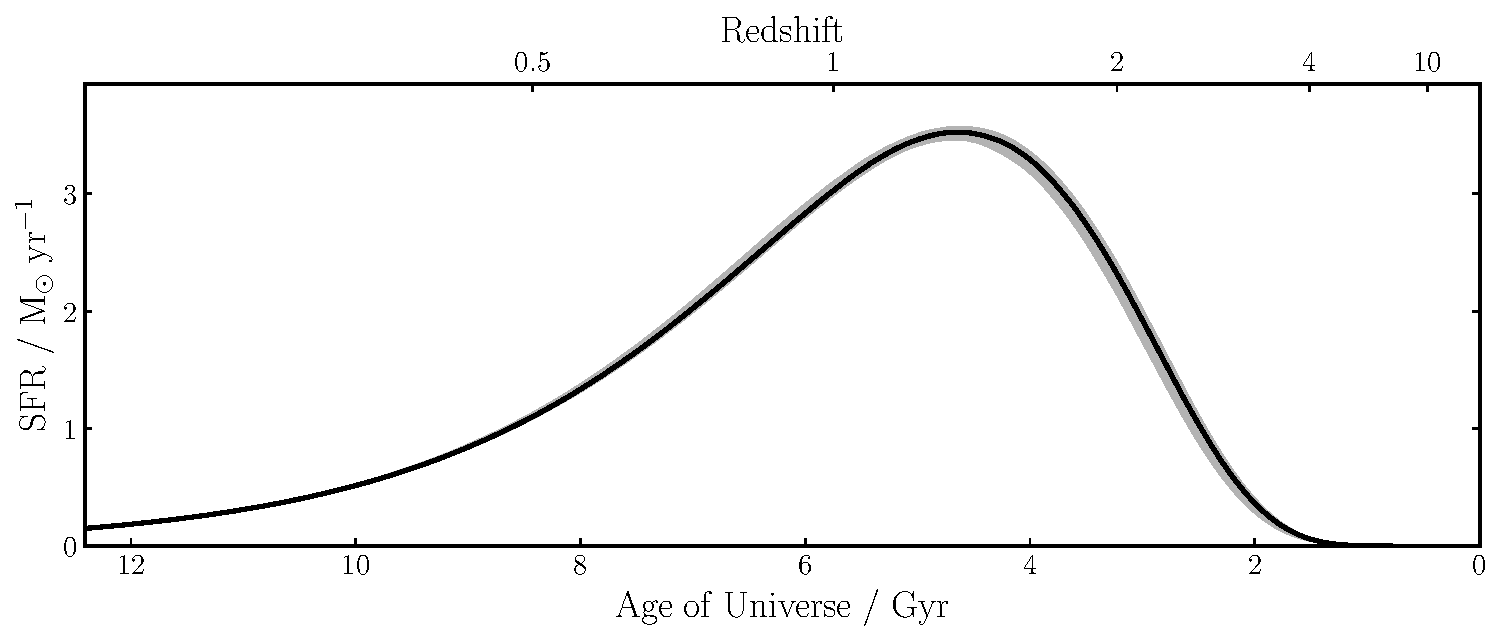
\includegraphics[width=0.9\textwidth]{../pipes/plots/exponential_burst_final/phil_model_2_sfh.pdf}
%   \caption{A priori and posterior SFH.}
%   \label{}
% \end{figure}
%
% \newpage
% \begin{figure}[h!]
%   \centering
%   \includegraphics[width=0.9\textwidth]{../pipes/plots/priors/phil_model_03_sfh.pdf}
%   \includegraphics[width=0.9\textwidth]{../pipes/plots/delayed_burst/phil_model_03_sfh.pdf}
%   \includegraphics[width=0.9\textwidth]{../pipes/plots/wide_delayed_burst/phil_model_03_sfh.pdf}
%   \caption{A priori and posterior SFH.}
%   \label{}
% \end{figure}
%
% \newpage
% \begin{figure}[h!]
%   \centering
%   \includegraphics[width=0.9\textwidth]{../pipes/plots/priors/phil_model_04_sfh.pdf}
%   \includegraphics[width=0.9\textwidth]{../pipes/plots/lognormal_burst/phil_model_04_sfh.pdf}
%   \includegraphics[width=0.9\textwidth]{../pipes/plots/wide_lognormal_burst/phil_model_04_sfh.pdf}
%   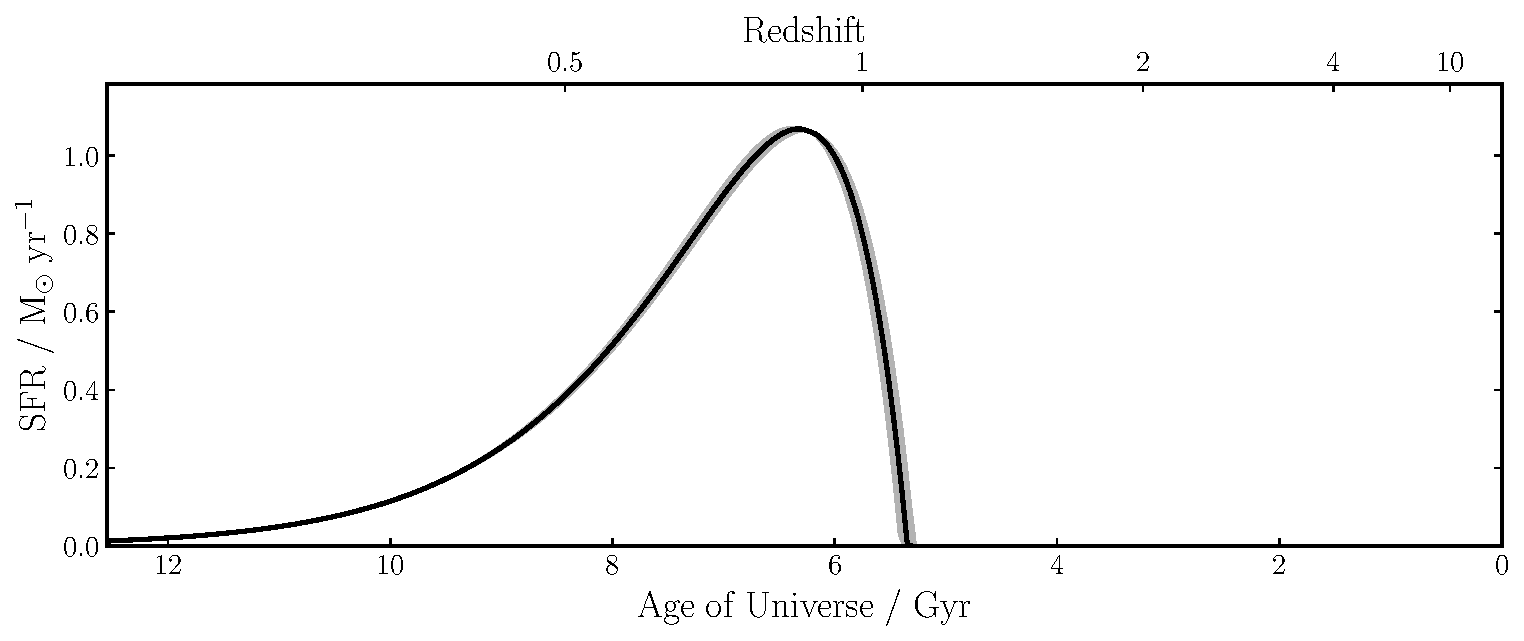
\includegraphics[width=0.9\textwidth]{../pipes/plots/exponential_burst_final/phil_model_4_sfh.pdf}
%   \caption{A priori and posterior SFH.}
%   \label{}
% \end{figure}
%
% \newpage
% \begin{figure}[h!]
%   \centering
%   \includegraphics[width=0.9\textwidth]{../pipes/plots/priors/phil_model_05_sfh.pdf}
%   \includegraphics[width=0.9\textwidth]{../pipes/plots/exponential_noburst/phil_model_05_sfh.pdf}
%   \includegraphics[width=0.9\textwidth]{../pipes/plots/exponential_noburst/phil_model_05_sfh.pdf}
%   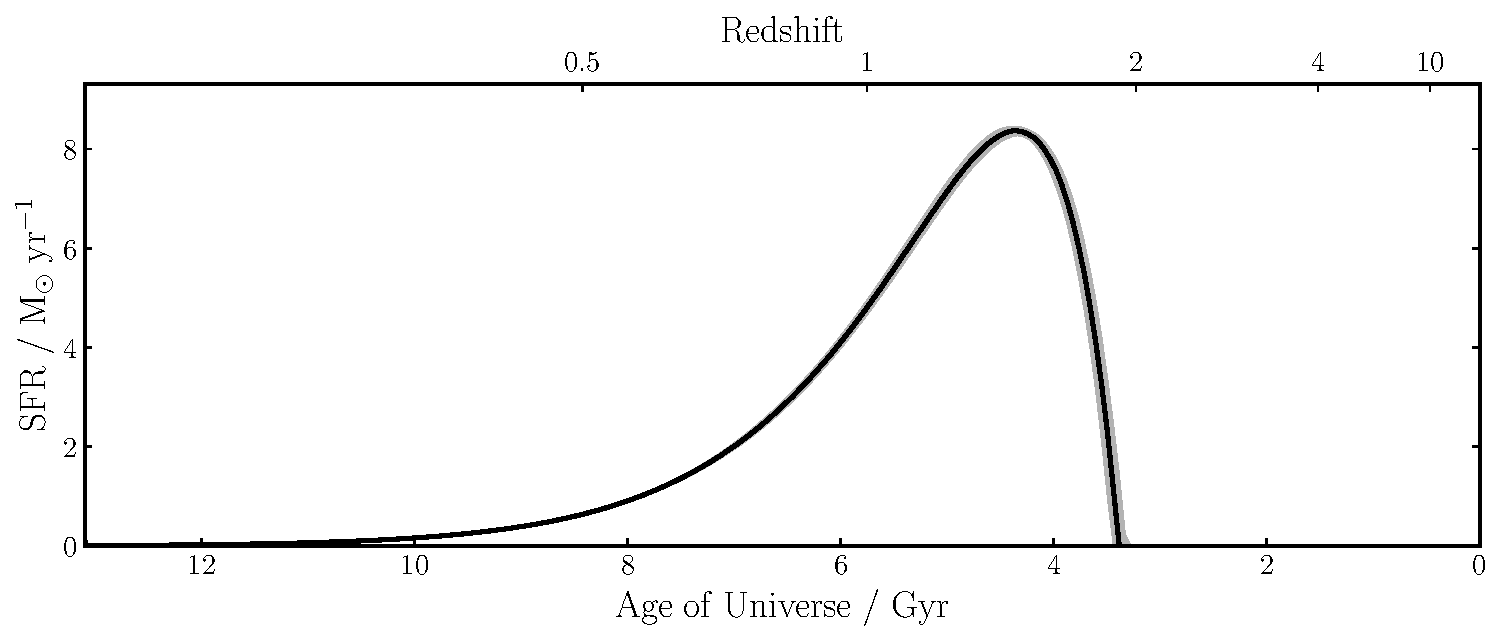
\includegraphics[width=0.9\textwidth]{../pipes/plots/delayed_burst_final/phil_model_5_sfh.pdf}
%   \caption{A priori and posterior SFH.}
%   \label{}
% \end{figure}
%
% \newpage
% \begin{figure}[h!]
%   \centering
%   \includegraphics[width=0.9\textwidth]{../pipes/plots/priors/phil_model_06_sfh.pdf}
%   \includegraphics[width=0.9\textwidth]{../pipes/plots/exponential_noburst/phil_model_06_sfh.pdf}
%   \includegraphics[width=0.9\textwidth]{../pipes/plots/wide_delayed_burst/phil_model_06_sfh.pdf}
%   \caption{A priori and posterior SFH.}
%   \label{}
% \end{figure}
%
% \newpage
% \begin{figure}[h!]
%   \centering
%   \includegraphics[width=0.9\textwidth]{../pipes/plots/priors/phil_model_07_sfh.pdf}
%   \includegraphics[width=0.9\textwidth]{../pipes/plots/exponential_burst/phil_model_07_sfh.pdf}
%   \includegraphics[width=0.9\textwidth]{../pipes/plots/wide_exponential_burst/phil_model_07_sfh.pdf}
%   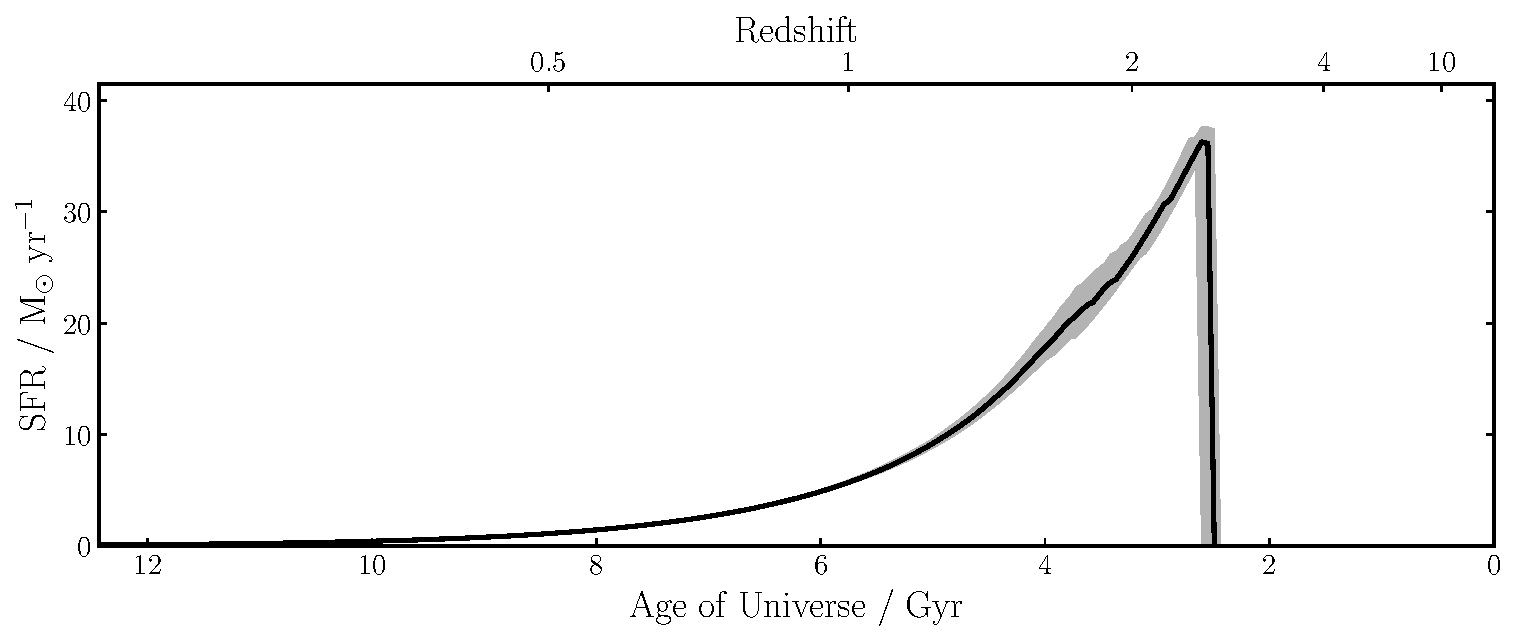
\includegraphics[width=0.9\textwidth]{../pipes/plots/delayed_burst_final/phil_model_7_sfh.pdf}
%   \caption{A priori and posterior SFH.}
%   \label{}
% \end{figure}
%
% \newpage
% \begin{figure}[h!]
%   \centering
%   \includegraphics[width=0.9\textwidth]{../pipes/plots/priors/phil_model_08_sfh.pdf}
%   \includegraphics[width=0.9\textwidth]{../pipes/plots/lognormal_burst/phil_model_08_sfh.pdf}
%   \includegraphics[width=0.9\textwidth]{../pipes/plots/wide_dblplaw_burst/phil_model_08_sfh.pdf}
%   \caption{A priori and posterior SFH.}
%   \label{}
% \end{figure}
%
% \newpage
% \begin{figure}[h!]
%   \centering
%   \includegraphics[width=0.9\textwidth]{../pipes/plots/priors/phil_model_09_sfh.pdf}
%   \includegraphics[width=0.9\textwidth]{../pipes/plots/exponential_burst/phil_model_09_sfh.pdf}
%   \includegraphics[width=0.9\textwidth]{../pipes/plots/wide_exponential_burst/phil_model_09_sfh.pdf}
%   \caption{A priori and posterior SFH.}
%   \label{}
% \end{figure}
%
% \newpage
% \begin{figure}[h!]
%   \centering
%   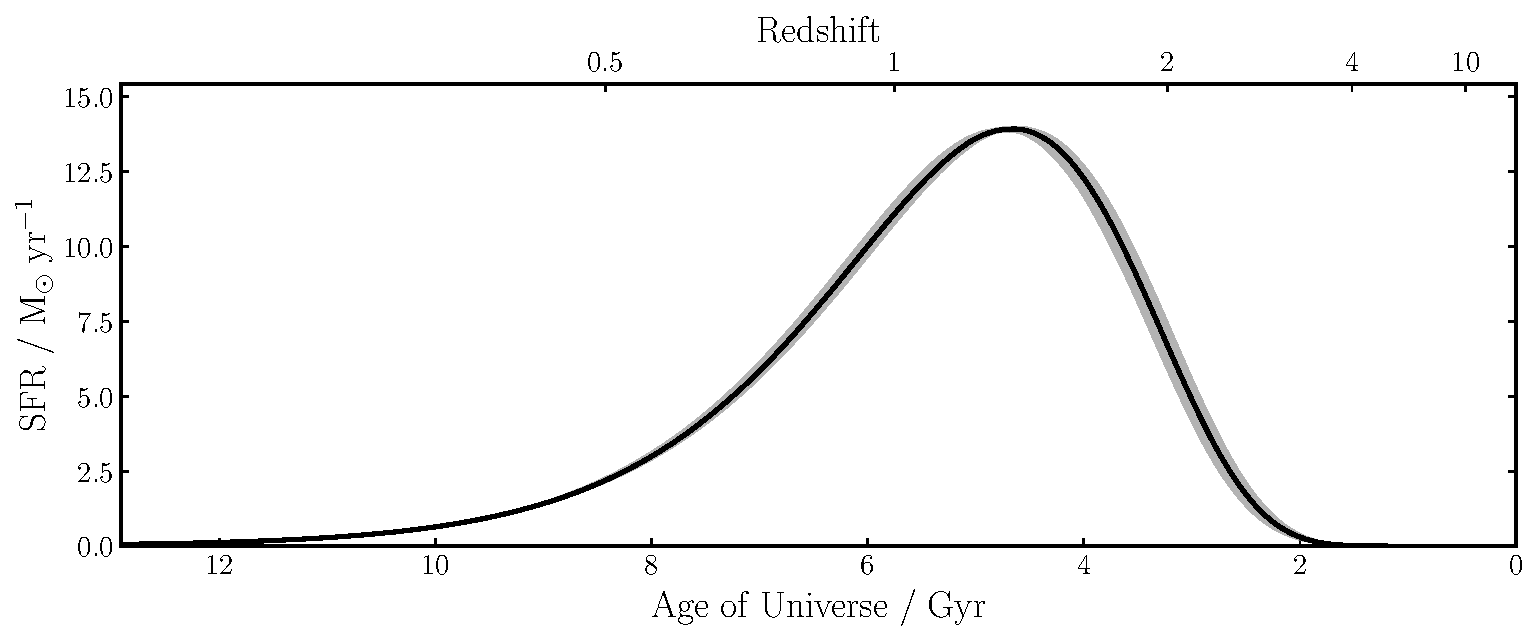
\includegraphics[width=0.9\textwidth]{../pipes/plots/priors/phil_model_10_sfh.pdf}
%   \includegraphics[width=0.9\textwidth]{../pipes/plots/exponential_burst/phil_model_10_sfh.pdf}
%   \includegraphics[width=0.9\textwidth]{../pipes/plots/wide_dblplaw_burst/phil_model_10_sfh.pdf}
%   \caption{A priori and posterior SFH.}
%   \label{}
% \end{figure}

\end{document}
